\documentclass[electronics,aricle,accept,pdftex,moreauthors]{Definitions/mdpi}

\firstpage{1} 
\makeatletter 
\setcounter{page}{\@firstpage} 
\makeatother
\pubvolume{1}
\issuenum{1}
\articlenumber{0}
\pubyear{2022}
\copyrightyear{2022}
\externaleditor{{Academic Editor: Yolanda Blanco Fernández } %MDPI: please add.
}
\datereceived{26 July 2022 } 
%\daterevised{} % Only for the journal Acoustics
\dateaccepted{1 September 2022} 
\datepublished{} 
%\datecorrected{} % Corrected papers include a "Corrected: XXX" date in the original paper.
%\dateretracted{} % Corrected papers include a "Retracted: XXX" date in the original paper.
\hreflink{https://doi.org/} % If needed use \linebreak
%\doinum{}
%--------------------------------------

\usepackage{amssymb}
\usepackage{amsmath}
\usepackage{epstopdf}
\usepackage{epsfig} 

\Title{RSU-aided Optimal Member Replacement Scheme with Improved Mobility Prediction for Vehicular Clouds In VANETs}

\TitleCitation{RSU-aided Optimal Member Replacement Scheme with Improved Mobility Prediction for Vehicular Clouds In VANETs}
%MDPI: title modified, please confirm.
\newcommand{\orcidauthorA}{0000-0003-3971-0715}
\newcommand{\orcidauthorB}{0000-0001-9410-7244}
\newcommand{\orcidauthorC}{0000-0001-7105-6026}
\newcommand{\orcidauthorE}{0000-0001-8578-8818}
\newcommand{\orcidauthorD}{0000-0002-0422-0647}

\Author{\hl{Youngju Nam} %MDPI: Please carefully check the accuracy of names and affiliations.
 \orcidA{}, Hyunseok Choi \orcidB{}, Yongje Shin \orcidC{}, Dick Mugerwa \orcidE{} and Euisin Lee *\orcidD{}}

\AuthorNames{Youngju Nam, Hyunseok Choi, Yongje Shin, Dick Mugerwa and Euisin Lee}

\AuthorCitation{Nam, Y.; Choi, H.; Shin, Y.; D. Mugerwa; Lee, E.}

\address[1]{School of Information and Communication Engineering, Chungbuk National University, Cheongju 28644, Korea; imnyj@chungbuk.ac.kr (Y.N.); hschoi@chungbuk.ac.kr (H.C.); yjshin@chungbuk.ac.kr (Y.S.); dmugerwa@chungbuk.ac.kr (D.M.)}

\corres{\hangafter=1 \hangindent=1.05em \hspace{-0.82em} Correspondence: eslee@chungbuk.ac.kr}

\abstract{The technique of vehicular clouds is considered an attractive approach in VANETs, because it provides a requester vehicle the ability to use resources of neighborhood vehicles (called cloud member vehicles) to construct a vehicular cloud to use next-generation vehicular applications during driving.
Generally, member vehicles can move along different routes from the route of the requester vehicle in intersections and, as a result, leave the vehicular cloud.
Then, the leaving member vehicle should be replaced by new member vehicles at intersections to reconstruct the vehicular cloud.
However, identifying optimal replacement vehicles among many vehicles at intersections is a very difficult task involving minimizing the waste of resources of vehicles due to their irregular mobility.
Thus, we propose an optimal member replacement scheme that finds optimal replacement vehicles through the improved mobility prediction of vehicles by borrowing the computational ability of RSUs on intersections.
The proposed scheme first makes an improved mobility prediction model by combining both the trajectory prediction of vehicles using the Markov model and the location prediction of vehicles using the Gaussian distribution.
Through the improved mobility prediction model, the proposed scheme then determines the leaving member vehicles and calculates their own leaving time.
Next, the proposed scheme addresses the problem to find optimal replacement vehicles to minimize the waste resource and solves it through an integer linear programming.
For the performance evaluation of the proposed scheme, we implement it in an NS-3 simulator, which includes the Manhattan mobility model, to reflect the mobility of vehicles on roads. 
Simulation results conducted in various environments verify that the proposed scheme achieves better performance than the existing scheme.}

\keyword{VANET; vehicular cloud; member replacement; mobility prediction; optimization}

\begin{document}
\section{Introduction}
Self-driving cars equipped with smart sensors and intelligent analysis tools can drive safely on their own trajectory with little or no human intervention.
With the recent rapid development of self-driving cars, testing and deployment have been strengthened in a much shorter time than previously expected.
Many companies, such as Tesla, Pony.ai, Waymo, Apple, Kia-Hyundai, Ford, Audi, Huawei, etc, are researching and developing autonomous vehicles with self-driving capabilities \cite{zhang2020}.
The autonomous vehicle is coming to reality with the effort of the companies.
The autonomous vehicle makes it unnecessary for not only passengers but also drivers to focus on driving all the time when on the road.
When full autonomation (i.e., level 5 \cite{yuan2018}) becomes a reality, they will need to find new entertainment during driving time.
Therefore, various and fresh applications are needed to meet these needs.

The advances in wireless networking technologies have innovated methods of entertainment (such as 5th generation (5G) cellular networks, Vehicular Ad-hoc NETworks (VANETs), etc).
Soon, users will use the autonomous vehicle as a device for new entertainment in vehicular networks.
However, due to the characteristics of vehicular networks (high speed, short communication range, dynamic topology, and limited storage and wireless resources), users may experience low-quality services from RSUs, such as long-term delays, buffering, and resolution reduction.
There are many challenges to be solved to improve the quality of user experience (QoE) and reduce network backhaul~traffic.

Many researchers have tried to solve this problem by using the vehicular cloud %\cite{Sibai2015, Meneguette2016, Meneguette2017b, Meneguette2017, Meneguette2017j, Choi2018, Lee2019, Mershad2013, Mershad2013j, Yu2013, Salahuddin2014, Lin2017}.
\cite{Meneguette2017j, Lin2017, Lee2019}.
Since the vehicular cloud immediately receives resource sharing from neighboring vehicles, its delay is relatively very small compared with Internet clouds.
In addition, because the vehicular cloud does not use resources of RSUs and cloud servers, network backhaul traffic can be reduced.
However, member vehicles in a vehicular cloud might leave the vehicular cloud while providing a cloud service to a requester vehicle desired for resources according to the vehicle trajectory.
Because the vehicular cloud is destroyed when the provision resources are less than the requested resources, it is essential to reconstruct the vehicular cloud by replacing the leaving member vehicle with new member vehicles.
Since the different types of vehicular clouds have different performances, we have to consider the two types of vehicular clouds: (1) the V2V vehicular cloud and (2)~the V2I vehicular cloud.
First, the V2V vehicular cloud uses only vehicles to construct the vehicular cloud \cite{Sibai2015, Meneguette2016, Meneguette2017b, Meneguette2017, Meneguette2017j, Choi2018}. % V2V 래퍼 논문
When the neighboring vehicles do not have enough resources to meet the requested demands, the requester vehicle, while driving, periodically broadcasts the request message to other neighbors until a new neighbor can provide the requested resources.
When the vehicular cloud is reconstructed, the probability of finding optimal replacement vehicles is low in terms of the available resource of the candidate member vehicles and the connectivity between the requester vehicle and the candidate member vehicles because the requester vehicle with a short communication range has a small number of candidates that can be replaced.
Additionally, the request messages that are periodically broadcast cause congestion of traffic in the vehicular network.
In the case of the V2I vehicular cloud, the requester vehicle uses a cloud server or infrastructure such as RSUs as a member of a vehicular cloud \cite{Lee2019, Mershad2013, Mershad2013j, Yu2013, Salahuddin2014, Lin2017}. 
In particular, RSUs have a wide range of communication and high computational capabilities \cite{Gao2018}.
If all requester vehicles want resources from an RSU, a bottleneck occurs and interferes with other services.
In addition, if all requester vehicles use a cloud server, it causes a significant amount of network backhaul traffic.
Fortunately, since the RSU has good capabilities, in order to find and replace the member vehicles that leave the vehicular cloud, we try to use only vehicles' information within the communication range of the RSU and the computational capabilities of the RSU.
Regarding the selection of a replacement member vehicle, because the two types of the vehicular cloud predict vehicles' connectivity based on simple movement information (such as position and speed) of the current vehicles, the prediction accuracy of the connectivity between vehicles is very low.
Accordingly, the connectivity may also be very low at the time that the vehicular cloud members are replaced \cite{Meneguette2017j}.
As a result, while another replacement member vehicle is being researched due to the prediction failure, the requester vehicle cannot receive a cloud service, resulting in an increase in delay.
In addition, by continuously finding additional replacement member vehicles, computational resources and traffic of the RSU are continuously consumed.

% 아래 부분 수정 필요. RSU-aided 용어 사용하여
To solve this problem, we propose an RSU-aided optimal member replacement scheme based on the improved mobility prediction of vehicles for vehicular clouds in VANETs.
First, the proposed scheme provides improved mobility prediction to enhance the accuracy of the connectivity prediction between vehicles in a vehicular cloud.
The connectivity prediction accuracy is improved by appropriately predicting the leaving member vehicles and the optimal replacement member vehicles through considering both the mobility prediction based on Gaussian probability and the trajectory prediction based on a Markov model.
% Through our improved mobility prediction, the proposed scheme then calculates the probability of the connection of vehicles in one direction and extends it into multiple directions to reflect intersections on roads.
% By the enhanced prediction accuracy, the proposed scheme can reduce the number of vehicular cloud reconstructions and as a result save delay and traffic that are consumed for the reconstruction of the vehicular cloud.
Next, the proposed scheme addresses the problem to identify optimal replacement member vehicles to minimize the wasted resources of vehicles.
The wasted resources are formulated based on the ratio of the size of the requested resource and the available resources of the vehicles that are selected as optimal replacement member vehicles in the restricted environment for the fairness of the wireless resources and energies.
Then, the problem is solved through an integer linear programming (ILP) in order to minimize the wasted resource, which excludes the resource that is allocated as each replacement member vehicle from its whole resource. 
% By determining optimal replacement member vehicles, the reliability and the service availability for vehicular cloud reconstruction are improved. 
% Moreover, network-wide available resources for other vehicular clouds are maximized by minimization the wasted resource through optimization.
To evaluate the performance of the proposed scheme, we compare it with one of the latest schemes, called SERVitES \cite{Meneguette2017j}.
% For the performance evaluation, we implements the simulation using NS3 with the enhanced Manhattan Mobility Model that vehicle has the accelerate with the Gaussian distribution and the directional shift with the Markov Model on the road.
Simulation results conducted in various environments demonstrate that the proposed scheme achieves better performance than SERVitES in terms of the wasted resource and the number of the cloud reconstruction.


The remainder of the paper is organized as follows. Section \ref{rel} examines the related works of this paper. Section \ref{net} describes the network model of this paper. Then, we describe the proposed scheme in detail in Section \ref{sec.op}. Simulation results are provided in Section \ref{per} to evaluate the performance of the proposed scheme. Section \ref{con} concludes the paper.


\section{Related Works} \label{rel}
Generally, the vehicular cloud is mainly categorized into V2I clouds and V2V clouds. In the V2I cloud schemes, the requester vehicle can construct a vehicular cloud with strong infrastructure support to reduce delay and improve cloud service stability. Many studies consider using roadside units (RSUs) which are deployed in urban scenarios to connect the requester vehicle and the Internet. Additionally, these RSUs have wide communication ranges and maintain connections with many requester vehicles \cite{Abdelhamid2017,Mershad2013,Jaiboon2017,Lin2017,Elahi2021,Rahman2018}.
%[23] Abdelhamid, S., Benkoczi, R., & Hassanein, H. S. (2017). Vehicular clouds: ubiquitous computing on wheels. In Emergent Computation (pp. 435-452). Springer, Cham.
%[28] Rahman, F. H., Wan, A. T., Newaz, S. S., & Suhaili, W. S. (2018, October). Vehicular Clustering: Fog Paradigm and Recent Advances. In 2018 IEEE 18th International Conference on Communication Technology (ICCT) (pp. 468-472). IEEE.
In \cite{Mershad2013}, the authors proposed a novel scheme that exploits the presence of RSUs to act as cloud directories that store information about mobile cloud servers called STARs. For each STAR, an RSU will store for the type of resources it offers, the attributes of each resource, and the required price per resource unit. Through this system, service discovery and service consuming delays are reduced, and the packet success ratio is improved.
In \cite{Lin2017} the author proposed a semi-Markov decision process (SMDP) model for vehicular cloud computing (VCC) resource allocation. It finds the optimal strategy of VCC resource allocation. The two additional features elaborate on the SMDP model and demonstrate different results from the original model. Its resource pool includes the RSUs provided by RSUs and the amount of RSUs of multiple vehicle types. Additionally, it considers different Poisson distributions for heterogeneous vehicle types.
In \cite{Jaiboon2017}, the authors proposed a mechanism of infotainment data distribution for vehicular networks using the RSU cloud. The system model and algorithms are suggested for vehicles, the RSU cloud, and the data center. The RSU cloud has the ability of cloud computing to solve the limitation of the traditional RSU for the efficiency of distributed infotainment messages. It can reduce the delay and throughput of vehicle communication through the RSU cloud and distribute infotainment messages.
In \cite{Elahi2021}, the authors proposed a vehicular cloud scenario where resources are allocated dynamically. They employed a vehicular cloud network using a roadside unit as the fixed coordinator and developed three resource allocation algorithms that aim to partially prioritize service cars, prioritize local cars, and reserve bandwidth for partially serviced cars. To allocate available resources dynamically, they consider a maximum portion of resources among all the competing vehicles and analyze the trade-off between serving a maximum number of vehicles or providing maximum quality of service.

%[24] Mershad, K., & Artail, H. (2013). Finding a STAR in a Vehicular Cloud. IEEE Intelligent transportation systems magazine, 5(2), 55-68.
%[25] Jaiboon, V., & Thaenthong, J. (2017, October). Infotainment data dissemination mechanism using RSU cloud based for vehicular networks. In 2017 9th International Conference on Information Technology and Electrical Engineering (ICITEE) (pp. 1-6). IEEE.
%[26] C. Lin, D. Deng, C. Yao, Resource allocation in vehicular cloud computing systems with heterogeneous vehicles and roadside units, IEEE Internet of Things Journal 5 (5) (2018) 3692{3700. doi:10.1109/JIOT.2017. 2690961.
%[27] M. M. Elahi, M. M. Rahman and M. M. Islam, "RSU-aided Mobility-aware Dynamic Resource Allocation for Vehicular Cloud Services," 2021 International Conference on Software Engineering & Computer Systems and 4th International Conference on Computational Science and Information Management (ICSECS-ICOCSIM), 2021, pp. 493-498, doi: 10.1109/ICSECS52883.2021.00096.

These V2I cloud schemes have several advantages, infinite resources, stable Internet connection, and low delay. However, these schemes have constraints. The infrastructure is essential to connect to the Internet, the limited communication range of RSU, and the high cost of using cellular networks. To overcome these V2I cloud constraints, the V2V cloud schemes are proposed.
In the V2V cloud schemes, vehicles search and allocate resources to each other through the information about their neighbor vehicles. The requester vehicle, which needs resources to construct its cloud for cloud service, sends a resource request to its neighbor vehicle. Neighbor vehicles cooperate to process the request and resource search. After searching for the requested resource, neighbor vehicles work together to allocate the resource to the requester vehicle. These schemes are performed among vehicles without any infrastructure \cite{Sibai2015,Meneguette2016,Meneguette2017b,Choi2018,Meneguette2017j,Meneguette2017}.
In \cite{Sibai2015}, the authors proposed a connectivity-aware service provision scheme where the service provider vehicle is selected based on several parameters such as the availability of the requested service and the mobility of the vehicles. It uses broadcasting to allow all neighbors to participate in the multi-hop resource search process to find many vehicles with enough resources.
In \cite{Meneguette2016}, the authors proposed a peer-to-peer protocol for the search and management of resources and services in the vehicular mobile cloud without depending on any external infrastructure called SMART. SMART selects the farthest neighbor vehicle from the resource search vehicle as an intermediate search vehicle called a controller and thus performs the multi-hop resource search process to larger regions by the controller.
In \cite{Meneguette2017b}, the authors proposed a new protocol for managing resources available in the vehicles within the cloud that promotes cooperation and collaboration among vehicles. It considers the one-hop connection time and selects the neighbor vehicle with the longest one-hop connection time as an intermediate search vehicle called a superpeer. It improves the availability of resources to the vehicle, increasing the amount of resources that can be consumed in the vehicle cloud.
In \cite{Meneguette2017j}, the authors proposed a protocol to assist in the search and management of resources in a vehicular cloud without depending on the support of roadside infrastructure. The vehicles have idle resources that can be made available to other vehicles by generating a moving cloud formed by a set of vehicles. To create this mobile cloud, they use clustering techniques to form efficient groups of vehicles. The cluster moves dynamically on the road, and vehicles can leave or join the cluster according to their proximity and speed.
In \cite{Choi2018}, the authors' proposed protocol uses a multi-hop connection time-based intermediate vehicle selection scheme to perform a multi-hop resource search and find vehicles with enough resources for a multi-hop vehicular cloud. To raise the vehicular cloud service availability, the proposed protocol allocates resources of vehicles based on the number of their neighbor vehicles and cloud service time for constructing a multi-hop vehicular cloud.

% [11] R. E. Siba, T. Atchian, J. B. Abdo, R. Tawil, and J. Demerjian, “Connectivity-aware service provision in vehicular cloud,” in Proc. Of the International Conference on Cloud Technologies and Applications(CloudTech), pp. 1-5, June 2015.
% [12] R. Meneguette, A. Boukerche, and R. De Grande, “SMART: an efficient resource search and management scheme for vehicular cloud-connected system,” in 2016 IEEE Global Communications Conference: Mobile and Wireless Networks (Globecom2016 MWN), Washington, USA, Dec.
% [13] R. Meneguette and A. Boukerche, “Peer-to-peer Protocol for Allocated Resources in Vehicular Cloud Based on V2V Communication,” in 2017 IEEE Wireless Communications and Networking Conference (WCNC), San Francisco, CA, USA, Mar.
% [14] H. Choi, Y. Nam, J. Bang, and E. Lee, “Multi-hop vehicular cloud construction with connection time based resource allocation in VANETs,” 2018 24th Asia-Pacific Conference on Communications (APCC). 05, May 2017.
% [15] R. Meneguette, A. Boukerche, "SERVitEs: An efficient search and allocation resource protocol based on V2V communication for vehicular cloud", Computer Networks, vol. 123, pp. 104-118, Aug. 2017.

These V2V cloud schemes have large scalability because they only communicate with each other and do not need any special nodes, such as RSUs, on roads. Thus, the requester vehicle can use cloud service while it is traveling to its destination. However, these schemes have several problems. First, vehicles have various mobility. This causes frequent topology changes. Second, the vehicular cloud is constructed over the multi-hop communication range. It causes weak connections among vehicles. Third, each vehicle has limited resources. For these reasons, the vehicular cloud construction is more complex, and it is repeatedly destroyed in urban scenarios, including those with many intersections. As a result, this reduces the cloud service stability.

As examined before, most studies are only focused on the vehicular cloud construction, and they restart the whole process of the vehicular cloud construction when the vehicular cloud is destroyed due to member vehicles leaving. 
Thus, if there are candidate vehicles to replace the leaving member vehicles, the vehicular cloud can be reconstructed rapidly. 
As one of the optimized vehicular cloud reconstruction methods, we only exploit the computing capability of RSUs, which have a large communication range, to overcome the limited small communication range of vehicles at a low communication cost.
In this condition, the contributions of this paper are as follows.
\begin{itemize}
    \item To enhance the prediction accuracy of the connection time between vehicles in a vehicular cloud, we propose an improved mobility prediction based on Gaussian distribution considering the locations of vehicles after some time.
    Using the improved mobility prediction, we appropriately estimate the leaving member vehicles and the optimal replacement member vehicles by calculating the probability of the connection of vehicles in one direction.
    \item Furthermore, using Markov model, this probability of the connection of vehicles based on the improved prediction can be applied to multiple directions to reflect intersections on the roads.
    By enhancing prediction accuracy, the proposed scheme can reduce the number of vehicular cloud reconstructions needed and as a result, reduce the delay and traffic that are consumed for the reconstruction of the vehicular cloud.
    \item Based on this connection probability, we formulate the wasted resources to maximize the network-wide available resources for the other vehicular clouds by minimizing the wasted resources through optimization.
    We formulate the wasted resources as the value of consideration for the ratio of the requested resources and available resources for optimal replacement of member vehicles of a vehicular cloud in the restricted environment for the fairness of wireless resources and energy.
    \item Then, to optimize the wasted resource to select the replacement vehicles with stable connectivity, we solve the problem using ILP.
    By determining optimal replacement member vehicles, the reliability and the service availability for vehicular cloud reconstruction are improved.
    \item For the performance evaluation, we implement the simulation using NS3 with the enhanced Manhattan mobility model such that vehicles accelerate with the Gaussian distribution and directionally shift with the Markov Model on the road.
    Simulation results are conducted in various environments to compare the performance of the proposed scheme with SERVitES in terms of the wasted resource and the number of the cloud reconstruction.
\end{itemize}

% We propose an optimal member replacement scheme considering the enhanced prediction of vehicle mobility in the multi-direction road scenario within the communication range of RSUs.
% To choose candidate vehicles with stable connectivity as a replacement vehicle, we predict the distance between two vehicles after a given time based on the Gaussian distribution.
% Using this prediction, we predict the connection probability between two vehicles after the given time based on the Markov Model in the multi-direction road scenario.
% Based on this connection probability, we formulate the wasted resource for optimization.
% Then, to optimize the wasted resource to select the replacement vehicles with stable connectivity, we solve the problem using ILP.
% To evaluate the performance of the proposed scheme, we compare the proposed scheme with SERVitES in terms of the wasted resource and the number of the cloud reconstruction in the enhanced Manhattan Mobility Model.

%-------------------------------------------------------------------------------------
%제안방안 개요 + Contribution
%-------------------------------------------------------------------------------------


% vehicular cloud는 주로 V2I cloud와 V2V cloud로 나뉜다.
%   V2V
%   V2I
% 제안 방안

\section{Network Model and Scheme Overview} \label{net}


In this section, we present the network model of the proposed scheme for a vehicular network and its overview.
As the network model, we consider that a number of vehicles move on roads according to their own traveling routes toward their own destinations.
There are intersections on the roads, and as a result each vehicle will pass multiple intersections until it arrives at its destination.
% 아래 레퍼런스로 다음 논문 추가 필요
% Z. Gao, D. Chen, S. Cai, and H. Wu, "Optimal and Greedy Algorithms for the One-Dimensional RSU Deployment Problem With New Model," IEEE Transactions on Vehicular Technology, Vo. 67, No. 8, pp. 7643-7657, Aug. 2018.
% H. Yu, R. Liu, Z. Li, Y. Ren, and H. Jiang, "An RSU Deployment Strategy Based on Traffic Demand in Vehicular Ad Hoc Networks (VANETs)," IEEE Internet of Things Journal, Vol. 9, No. 9, pp. 6496-6505, May 2022.
We assume that each intersection has an RSU to provide Internet connections to vehicles within its communication coverage, as many studies \cite{Gao2018, Yu2022} have mentioned similarly.
When every vehicle enters within the communication coverage of an RSU, it sends a beacon message with its ID, location, mobility, and resource information to the RSU periodically.
In particular, the mobility information of a vehicle includes its speed and the probability of its traveling route, and the resource information of the vehicle includes its resource type and its available amount.

In the situation of the network model, when a vehicle wants to use a vehicular application requiring a large amount of resource, it constructs a vehicular cloud for supporting the application.
In this paper, we call a vehicle that intends to construct a vehicular cloud a requester vehicle.
To construct a vehicular cloud, a requester vehicle sends a request message with the information of the requested resource amount and a request time to borrow the resources necessary for the vehicular cloud to its neighborhood vehicles. 
On receiving the request message, every neighborhood vehicle sends a reply message with its ID, location, mobility, and resource information to the requester vehicle.
Based on the information in all of the reply messages from neighborhood vehicles, the requester vehicle selects member vehicles among them for the vehicular cloud.
% 아래 레퍼런스에 vehicular cloud 구성하는 우리 이전 논문과 다른 논문 포함하기
As in the previous papers~\cite{Lee2019, Choi2018, Meneguette2017j}, in the proposed scheme, the member vehicles are determined to meet the conditions for constructing the vehicular cloud, including that both the expected connection time between the requester vehicle and each member vehicle is longer than the request time and the total summation of the resource from all member vehicles is larger than the requested resource amount.
Then, the requester vehicle stores the information of each member vehicle in each entry of a member vehicle table for the vehicular cloud.
To know the member vehicle selection, the requester vehicle sends a selection message to each of the member vehicles.
Upon receiving the section message, every member vehicle recognizes itself as a member vehicle for the vehicular cloud and uses the resource for operating the vehicular cloud.
By this process, if the vehicular cloud is constructed, the requester vehicle periodically asks for and receives a beacon message from all of the member vehicles to maintain the vehicular cloud until the vehicular cloud is finished completely.

% 차량들은 정기적으로 RSU에게 비콘 메시지를 통하여 이동성 정보 전달
% 요청 차량의 의의
% 요청 차량에 의한 클라우드 생성
%   주변 차량에게 정보 요청 > 리소스, 이동성 정보(속도, 경로에 대한 확률) 반환
%   기대 연결 시간이 요청 리소스 시간 충분한지 + 가용 리소스의 조합이 요청 리소스와 가까운지
%   메시지를 보내 차량 클라우드 생성
% 유지를 위한 정기적인 비콘 메시지
%   정기적인 리소스 공유를 하면서 패킷에 차량의 이동성 정보를 넣어 계속 갱신

% 아래 두 문장은 굳이 필요없음.
%   이동성으로 인하여 당장 클라우드를 이탈할 때, Leave message를 보내고 이탈
% 서비스 만족이나 제공 리소스 량이 요구량을 못 맞출 때 NACK(?)를 보내서 클라우드 해체

While using the vehicle cloud, the requester vehicle might move along a road with its member vehicles together.
Usually, they pass several intersections until they arrive at their own destinations.
When the requester vehicle with its member vehicles approaches an intersection, they might move along different roads from the intersection according to their own traveling routes. 
As a result, some of the member vehicles could leave the vehicular cloud because their traveling routes might be
different from that of the requester vehicle. 
Accordingly, the vehicular cloud for the requester vehicle is destroyed due to the leaving member vehicles at the intersection, because it can no longer use resources provided by them for the vehicular cloud.
Thus, in an intersection, the vehicular cloud that includes the requester vehicle needs to replace the leaving member vehicles with the replacement vehicles that are selected by the RSU.
The replace member vehicles will be selected from vehicles that move along the same traveling route as that of the requester vehicle from the~intersection.

% to maximize the stability of cloud services and to minimize the wasted resources
With regard to the member vehicle replacement, one of the most challenging issues is to find optimal replacement vehicles to replace the leaving member vehicles. 
To select the optimal replacement vehicles, the vehicular cloud sends the request message when it enters the communication range of the RSU, as shown in Figure \ref{FigOverview}a.
Since the RSU has information about all the vehicles within a longer communication range than the vehicle, it has more candidate vehicles to select the optimal replacement vehicles.
To maximize the stability of the cloud service from a vehicular cloud, replacement vehicles should have enough resources for the vehicular cloud to prevent its destruction due to a lack of resources.
Then, we focus on the resource of vehicles for the optimization, because the resources of vehicles are the most important and necessary key factor to construct vehicular clouds.
The waste of resources significantly affects the construction and the reconstruction of vehicular clouds. 
Thus, the proposed scheme achieves the minimization of wasted resources when determining optimal replacement vehicles to replace the leaving member vehicles.
To decide on optimal replacement vehicles to achieve the minimization of the wasted resource, the proposed scheme exploits the resource and mobility information of vehicles.
After the RSU selects the optimal replacement vehicle, it sends a selection message to each selected replacement vehicle, which includes the replacement time and information about the requester vehicle, and the replacement vehicles with the included information send a join message to the requester vehicle to join the vehicular cloud at the replacement time as shown in Figure \ref{FigOverview}b.
In the next Section \ref{sec.op}, we describe the proposed scheme to select optimal replacement vehicles based on the resource and mobility information of vehicles under our network model in detail.
Table \ref{table1} shows notations used for the proposed scheme in this paper.
% the stability of cloud services과 the wasted resources를 달성하기 위한 optimal new member vehicles의 선정시에 차량들의 mobility 정보와 resource 정보를 기반으로 한다.
% Mobility 정보를 통해서 the stability of cloud services 달성
% resource 정보를 통해서 the wasted resources 달성


% RSU 범위에 들어간 요청 차량은 멤버 정보를 RSU에 전송
% RSU는 이탈 확률 및 시간 계산하여 통신 범위 내에 이탈 시간에 요청 차량에게 연결될 수 있는 가용 리소스가 충분한 교체 차량 검색
% 교체 차량들에게 요청 차량의 정보와 교체 되어야하는 시간이 포함된 SELECT 메세지 보냄
% SELECT message 받은 차는 해당 시간에 요청 차량에게 Join 메세지를 보내어 cloud 참여
% "+ as shown in Figure \ref{FigOverview}(b)"
% wasted resource를 최소화하기 위해, 교체 차량이 들어가면 나가기로 되어 있던 차량에게 요청 차량이 nack 메세지를 보내어 나가게 만듦
% 요청 차량은 최적화된 리소스의 량을 제공받음

\begin{figure}[H]
    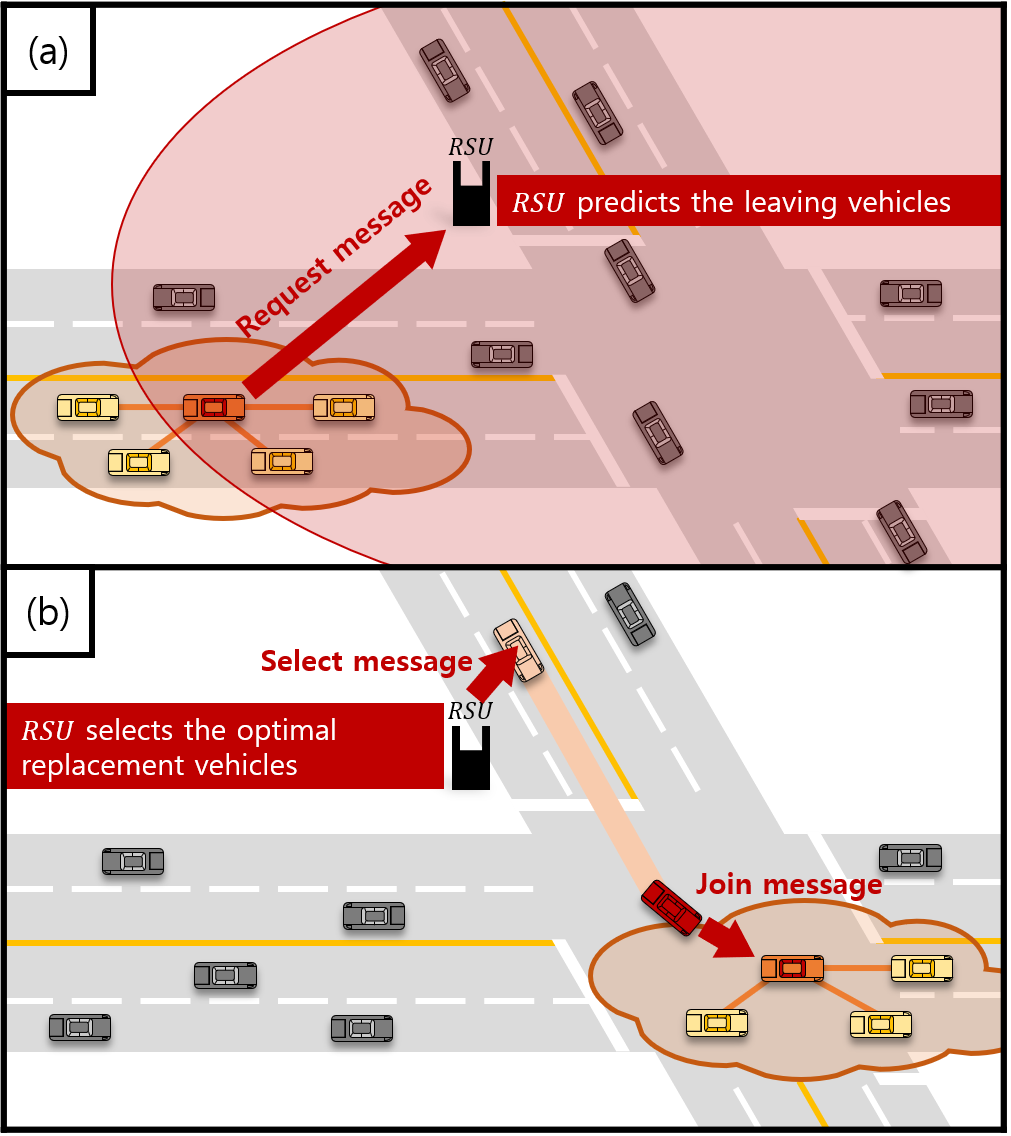
\includegraphics[width=7cm]{./figures/figure1.png}
    \caption{\hl{The} %MDPI: we move all tables and figures after its first citation. please confirm
 network model and scheme overview: (\textbf{a}) when a vehicular cloud enters into the communication coverage of a RSU, the requester vehicle sends a request message to the RSU to carry out the member vehicle replacement, and (\textbf{b}) the RSU selects the optimal replacement vehicles, and the vehicular cloud is reconstructed with the optimal replacement vehicles.}
    \label{FigOverview}
\end{figure}




\begin{table}[H] % table1
    \caption{\hl{Notations} %MDPI: Please confirm if this is placed here as table 1 and not in the Notations section in back matter?.
 used in the proposed scheme.}
\setlength{\cellWidtha}{\textwidth/2-2\tabcolsep-1in}
\setlength{\cellWidthb}{\textwidth/2-2\tabcolsep+1in}
\scalebox{1}[1]{\begin{tabularx}{\textwidth}{>{\centering\arraybackslash}m{\cellWidtha}>{\raggedright\arraybackslash}m{\cellWidthb}}
        \toprule
        \textbf{Notation} & \textbf{Description} \\
        \midrule
        $t_{n}$ & $n$-th time slot \\
        $\Delta T$ & one time slot \\
        $\Delta t$ & unit time \\ 
        $m$ & the number of unit time \\
        $v^{(k)}_{x}$ & x-axis velocity at the $k$-th unit step between $t_{n-1}$ and $t_{n}$ \\
        $x^{(k)}$ & x-axis location at the $k$-th unit step between $t_{n-1}$ and $t_{n}$ \\
        $\varepsilon^{(k)}_{x}$ & x-axis acceleration at the $k$-th unit step between $t_{n-1}$ and $t_{n}$ \\
        $\mu_{x}$ & the mean of the x-axis location at $t_{n}$ \\
        $\sigma_{x}$ & the standard deviation of the x-axis location at $t_{n}$ \\
        $\mu_{d}(\alpha,\beta)$ & the mean of the distance between $\alpha$ and $\beta$ at $t_{n}$ \\
        $\sigma_{d}(\alpha,\beta)$ & the standard deviation of the distance between $\alpha$ and $\beta$ at $t_{n}$ \\
        $Pr_{conn}^{[\alpha,\beta]}(t_{n})$ & the probability of connection between $\alpha$ and $\beta$ at $t_{n}$ \\
        $Pr[\alpha^{s}_{n}((x_{n},y_{n}))]$ & the probability of the vehicle $\alpha$ reaching $(x_{n}, y_{n})$ at $t_{n}$ \\
        $\theta_{th}$ & the threshold value of determining that two nodes are connected \\
        $R_{need}^{req}(t)$ & \begin{tabular}{@{}l@{}} the expected needed resources of the vehicular cloud \\ due to the leaving member vehicles \end{tabular} \\
        $R_{avail}^{j}$ & the available resource of the $j$-th member vehicle \\
        $R_{req}$ & the requested resource by the requester vehicle $req$ \\
        $r_{wasted}^{req}(t)$ & the percentage of the wasted resources at time $t$ \\
        $\xi^{req,l}(t)$ & \begin{tabular}{@{}l@{}} determinant value whether the vehicle $l$ is selected \\ as a replacement vehicle for $req$ at $t$ \end{tabular} \\
        $T_{service}^{req}$ & valid time of the cloud service that is requested by $req$ \\
        $\eta_{rel}$ & weight value to focus on the stability of the cloud service \\
        $\eta_{wasted}$ & weight value to focus on minimizing the wasted resource \\
        \bottomrule
    \end{tabularx}}
    \label{table1}
\end{table}


\section{The Optimized Cloud Member Replacement Scheme} \label{sec.op}
This section describes an optimized cloud member replacement scheme for determining new member vehicles to replace the leaving member vehicles in order to maximize the stability of cloud services and to minimize the wasted resources.
A vehicle demands resources from neighboring vehicles that cannot be solved by itself and becomes a requester vehicle.
Neighboring vehicles provide information about their available resources.
The available resource information that is received from the neighbor is used to determine whether the requested resource is satisfied.
If the sum of available resources of neighboring vehicles is less than the requested resources, the vehicular cloud service cannot be executed, so the requester vehicle continuously requests resources from other neighboring vehicles while moving.
If the sum of available resources of neighboring vehicles is bigger than the requested resources, the requester vehicle selects neighboring vehicles to be used as vehicular cloud members according to the requested resources.
A neighboring vehicle that is selected as a vehicular cloud member continuously sends the mobility information to the requester vehicle through a beacon message in order to maintain connectivity.
When the requester vehicle enters the RSU's communication range, it provides the information regarding the vehicular cloud members to the RSU.
To maintain the cloud service of the requester vehicle, the RSU selects the optimal replacement vehicles and replaces the leaving member vehicle among the vehicular cloud members in terms of maximizing the stability of the cloud service and saving the wasted resources.
To do this, we first formulate the connection probability between vehicles after the time $t$ in Section \ref{sec.op1}.
Because the RSU is deployed at each intersection, the connection probability between vehicles after time $t$ is redefined in Section \ref{sec.op2} using the Markov model and considering the trajectory probability of the vehicle at each intersection.
In Section \ref{sec.op3}, we formulate the wasted resources using the connection probability based on resources that are insufficient due to the leaving member vehicles among the vehicular cloud members and resources that are replaced by the replacement candidate vehicles.
In Section \ref{sec.op4}, we solve the optimization problem using ILP to maximize the cloud service stability and to minimize the wasted resources.

\subsection{Probability of the Connection in One Direction} \label{sec.op1}

This section describes the probability of connecting the two vehicles according to $t_{n}$ on a one-direction road, as shown in Figure \ref{FigOne}. In order to calculate the connection probability between vehicles after time $t_{n}$, the location probability of vehicles at time $t_{n}$ must first be calculated.
Let $\Delta t$ be the unit step time between time $t_{n-1}$ and time $t_{n}$, $\Delta T=t_{n}-t_{n-1}=m\Delta t$, and $m$ denote the number of unit time.
The speed of the vehicle is legally limited, and the acceleration of the autonomous vehicle is limited to [$-$5, 5] $m/s^{2}$ for user convenience \cite{Robert2018, Yen2020}.
The velocity of vehicles is assumed to follow a random distribution at time $t_{n}$.
Therefore, within the limit not exceeding the speed limit, the velocity can be regarded as a uniform motion, and the acceleration can be regarded as a series of white Gaussian noise with a constant variance $\varepsilon$ during unit time $\Delta t$ \cite{jiang2019}.
For vehicle $i$ at the $k$-th unit step between time $t_{n-1}$ and time $t_{n}$, the x-axis velocity component is denoted by $v^{(k)}_{x}$, and the x-axis location component is denoted by $x^{(k)}$:
\begin{align}
    v_{x}^{(k)}&=v_{x}^{(0)}+ \sum\limits_{i=1}^{k}\varepsilon_{x}^{(i)}\Delta t,\\
    x^{(k)}&=x^{(0)}+k \Delta tv_{x}^{(k)}+\frac{1}{2}\sum\limits_{i=1}^{k}(2k-2i+1)\varepsilon_{x}^{(i)}\Delta t^{2},
\end{align}
where $\varepsilon^{(k)}_{x}$ is the acceleration component in \cite{lin2012}.
The arguments of Gaussian distribution at $t_{n}$ are achieved as:
\begin{align}
    \mu_{x}&=x_{n-1}+v_{(n-1)}^{x}m\Delta t,\\
    \sigma_{x}^{2}&=\frac{(4m^{3}-m)\xi\Delta t^{4}}{12},
\end{align}
where $(x_{n-1},y_{n-1})$ denotes the location at time $t_{n-1}$.
The expressions of the y-axis and z-axis are similar to the results of the x-axis.
Thus, based on the location $(x_{n-1},y_{n-1})$ at time $t_{n-1}$, the probability density function to arrive at $(x_{n},y_{n})$ is achieved as:
\begin{equation}
    \begin{split}
        p\{(x_{n}, y_{n})\vert (x_{n-1},y_{n-1})\}=\frac{1}{2\pi\sigma^{2}}\exp^{\left(-\frac{1}{2\sigma^{2}}\left[(x_{n}-\mu_{x})^{2}+(y_{n}-\mu_{y})^{2}\right]\right)}.
    \end{split}
\end{equation}

Using this probability, the arguments of Gaussian distribution at time $t_{n-1}$ can be redefined in terms of the distance between vehicle $\alpha$ and vehicle $\beta$, as follows:
\begin{align}
    \mu_{d}(\alpha,\beta)=&\left(\mu_{x}^{\alpha}-\mu_{x}^{\beta}\right)^{2}+\left(\mu_{y}^{\alpha}-\mu_{y}^{\beta}\right)^{2},\\
    \begin{split}
        \sigma_{d}^{2}(\alpha,\beta)=&\frac{\Delta t^{4}}{4}\times E\left[\sum_{i=1}^{m}(2i-1)^{4}\left( (\varepsilon^{(k)2}_{\alpha,x}-\varepsilon^{(k)2}_{\beta,x})^{2} + (\varepsilon^{(k)2}_{\alpha,y}-\varepsilon^{(k)2}_{\beta,y})^{2}\right) \right],
    \end{split}
\end{align}
where the arguments of Gaussian distribution of vehicle $\alpha$ are $\mu_{x}^{\alpha}, \mu_{y}^{\alpha}, \varepsilon^{(k)}_{\alpha,x}, \varepsilon^{(k)}_{\alpha,y}$, and the arguments of Gaussian distribution of vehicle $\beta$ are $\mu_{x}^{\beta}, \mu_{y}^{\beta}, \varepsilon^{(k)}_{\beta,x}, and \varepsilon^{(k)}_{\beta,y}$.
Therefore, based on the distance $d_{n-1}$ between vehicle $\alpha$ and vehicle $\beta$ at time $t_{n-1}$, the probability density function to reach $d_{\gamma}$ is achieved as:
\begin{equation} \begin{split}
    p\{d_{n}(\alpha,\beta)=d_{\gamma}\vert d_{n-1}(\alpha,\beta)\}=\frac{1}{2\pi\sigma^{2}}\exp^{\left(-\frac{1}{2\sigma^{2}}\left[(d_{n}-\mu_{d}(\alpha,\beta))^{2}\right]\right)}.
\end{split} \end{equation}


The probability that the distance between the two vehicles is less than the communication range $range_{V2V}$ at time $t_{n}$ using an integral under $d_{n}$ is as follows:

\begin{equation}
    Pr_{conn}^{[\alpha,\beta]}(t_{n})=\int_{0}^{range_{V2V}} p\{d_{n}(\alpha,\beta)=q\vert d_{n-1}(\alpha,\beta)\}\, dq
\end{equation}

Using the obtained connection probability between the two vehicles at time $t_{n}$, the leaving time of the vehicular cloud member and the entry time of the candidate vehicle to be replaced can be estimated.

\begin{figure}[H]
    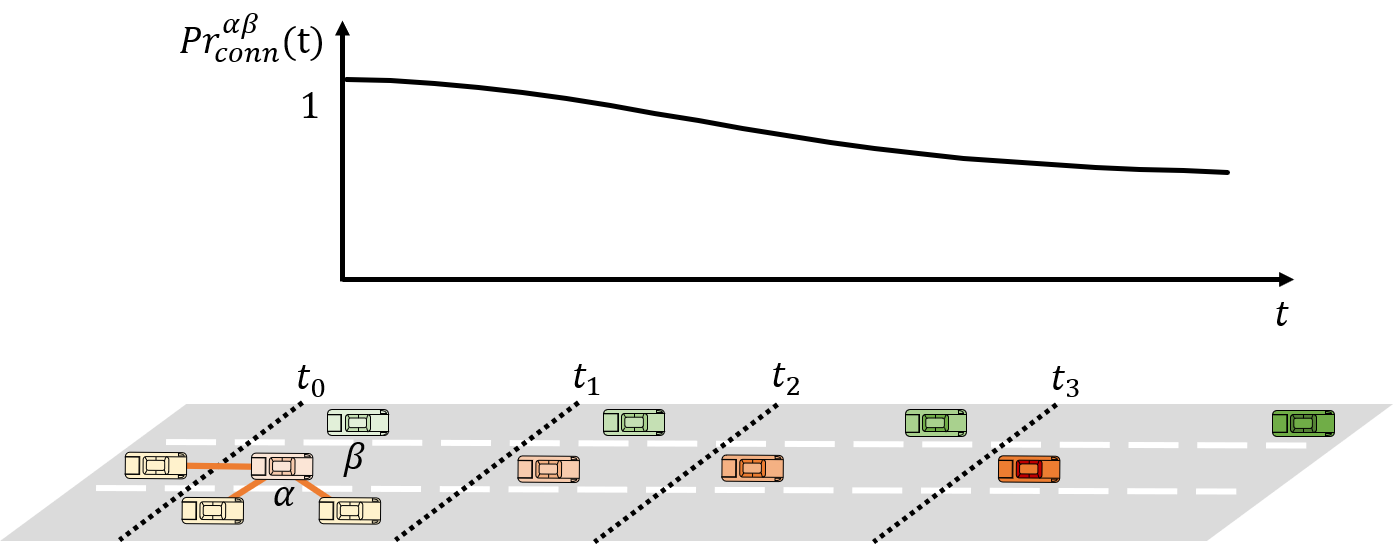
\includegraphics[width=13cm]{./figures/figure2.png}
    \caption{Probability of a connection in one direction.}
    \label{FigOne}
\end{figure}


\subsection{Probability of the Connection in Multiple Directions} \label{sec.op2}

This section describes the probability of connecting two vehicles according to $t_{n}$ on a multi-direction road, as shown in Figure \ref{FigMulti}.
A vehicle suffers a number of multi-direction paths within the communication range of RSUs installed at each intersection, so the connection probability between the two vehicles at time $t_{n}$ should be calculated in consideration of the trajectory probability of each vehicle.
The trajectory probability of the vehicle can be calculated using the Markov model that estimates the trajectory based on historical data.
RSUs, who receive mobility information that is sent by the vehicle, send the information to the movement management server to manage the historical data of each vehicle, thereby obtaining the trajectory probability for each vehicle.
The Markov model is affected by the order number because a big order has high complexity.
The trajectory probability of a 1st-order Markov model is as follows:
\begin{equation}
    {p}_{i(i+1)}=Pr(L_{(i+1)}|L_i)=\frac{X(L_i,L_{(i+1)})}{Z(L_i)},
\end{equation}
where ${p}_{i(i+1)}$ is the trajectory probability that is derived based on the number of times that the vehicle has moved to $L_{i+1}$ when it drives at $L_{i}$.
Through this probability, it is the 2nd-order Markov model that performs the calculation once more considering the situation before $L_{i}$, denoted as follows:
\begin{equation} \begin{split}
    {p}_{(i-1)i(i+1)}&=Pr(L_{(i+1)}|L_i,L_{(i-1)})=\frac{X(L_{(i+1)},L_i,L_{(i-1)})}{Z(L_i, L_{(i-1)})},
\end{split} \end{equation}
where ${p}_{(i-1)i(i+1)}$ is the trajectory probability that is derived based on the number of times that the vehicle has moved to $L_{i+1}$ when it drives at $L_{i}$ from $L_{i-1}$.
Depending on the order of the Markov model, the accuracy of the trajectory prediction increases but leads to a tremendous increase in complexity.
Therefore, we predict the trajectory using the 2nd-order Markov model.
In section A, we formulate the location probability according to the acceleration and velocity of the vehicle.
By mixing this location probability with the trajectory probability, if the location of vehicle $\alpha$ is $(x_{n-1}, y_{n-1})$ at time $t_{n-1}$, the probability of the vehicle reaching $(x_{n}, y_{n})$ at time $t_{n}$ when the vehicle selects the $s$-th path among $S$ paths is denoted as follows: 
\begin{equation}
    \begin{split}
        Pr[\alpha^{s}_{n}((x_{n},y_{n}))]=p\{(x_{n}, y_{n})\vert (x_{n-1}, y_{n-1})\} \times p^{\alpha}_{(n-1)n, s}.
    \end{split}
\end{equation}

Thus, the probability that the distance between vehicle $\alpha$ and vehicle $\beta$ is less than the communication range is calculated differently depending on the $s$-th path among $S$ paths.
The expected connection probability between the two vehicles at time $t_{n}$ considering the trajectory probability of each vehicle is denoted using the cumulative distribution function (CDF) as follows:
\begin{equation}
    Pr^{\alpha,\beta}_{conn}(t_{n})= \sum_{s=1}^{S}\left(p^{\alpha}_{s} \sum_{r=1}^{S}\left(p^{\beta}_{r}\times Pr_{conn}^{[\alpha^{s},\beta^{r}]} \right)\right).
\end{equation}

The connection probability between the two vehicles at time $t$ can determine whether to replace the cloud member, and replacement candidates can also be selected.

\begin{figure}[H]
    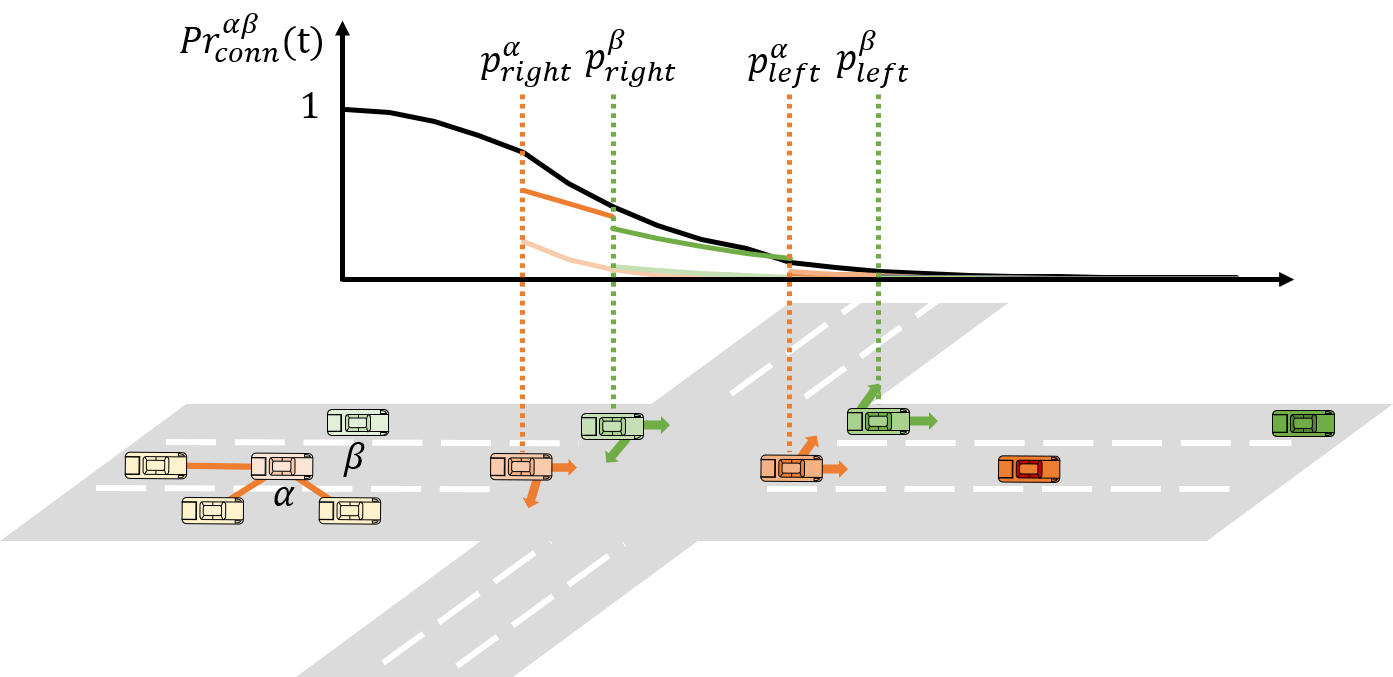
\includegraphics[width=13cm]{./figures/figure3.png}
    \caption{Probability of the connection in multiple directions.}
    \label{FigMulti}
\end{figure}

\subsection{Calculation of the Wasted Resources} \label{sec.op3}
When allocating the replacement vehicle to replace the vehicle that leaves the vehicular cloud at time $t$, the replacement vehicle consumes energy and resources to provide the cloud service.
In the case of a vehicle that has many available resources, many vehicles around will use the vehicle's resources.
The vehicle consumes a lot of energy and wireless resources (time slot, bandwidth, and channel) to share resources with many requester vehicles.
Therefore, for fairness to the usage of energy and radio resources, we assume that a vehicle that shares its available resources in one vehicular cloud does not share the remaining available resources in the other vehicular cloud.

When a vehicle is expected to leave the vehicular cloud, the RSU allocates an optimal replacement vehicle to the requester vehicle in order to maintain the cloud service based on the mobility and resource information of vehicles within the RSU's communication range.
The amount of resources that are insufficient due to the leaving member vehicles reduces the total provided resources of the vehicular cloud.
The vehicular cloud cannot be maintained when the total provided resources of the vehicular cloud are less than the requested resources by the requester vehicle $req$.
The expected needed resources $R_{need}(t)$, which are insufficient due to the leaving member vehicles, are denoted as follows:
\begin{equation} \begin{split}
    R_{need}^{req}(t)=&\sum_{j=1}^{J} \left( \delta(Pr^{req,j}_{conn}(t)<\theta_{th}) \times R_{avail}^{j} \right)- \left(\sum_{j=1}^{J} \left( R_{avail}^{j} \right) - R_{req}\right),
\end{split} \end{equation}
where $J$ is the total number of member vehicles in the vehicular cloud, $R_{avail}^{j}$ is the available resources of the $j$-th member vehicle, and $R_{req}$ is the requested resources by the requester vehicle $req$.
$\theta_{th}$ is derived from the optimization equation as a determinant.
When the probability that the $j$-th member vehicle leaves the vehicular cloud is greater than $\theta_{th}$, $\delta(Pr^{req,j}_{conn}(t)<\theta_{th})$ considers the member as the leaving member vehicle and has a value of 1.
Otherwise, it has a value of 0.

To maintain the vehicular cloud, the sum of the available resources $R_{avail}^{l}$ of the vehicle that is allocated as the $l$-th replacement vehicle must be greater than $R_{need}(t)$ at every time $t$.
However, when a vehicle with too many available resources is allocated as a replacement vehicle, the resources that remain after being provided to the requester vehicle cannot be shared to other vehicular clouds and are wasted.
If the ratio of $R_{need}(t)$ to the sum of the available resources of the allocated replacement vehicle is close to 1, the wasted resources can be minimized.
The percentage $r_{wasted}(t)$ of the wasted resources at time $t$ is denoted as~follows:
\begin{equation}
   \frac{1}{r_{wasted}^{req}(t)} =\frac{R_{need}^{req}(t)}{\sum_{l=1}^{L}\left( \xi^{req,l}(t) \times R_{avail}^{l}\right)},
\end{equation}
where $\xi^{req,l}(t)$ is a determinant and is 1 when the candidate vehicle $l$ is selected as a replacement vehicle for $req$ at time $t$. Otherwise, it has a value of zero.
$\frac{1}{r_{wasted}^{req}(t)}$ has a value of 1 or less because the sum of the available resources of the replacement vehicle must be greater than or equal to $R_{need}^{req}(t)$.

\subsection{The Optimization of the Wasted Resources} \label{sec.op4}
In order to stabilize the cloud services, the vehicle with the highest connection probability is selected as a replacement vehicle, and to minimize the wasted resources, the objective function is denoted as follows:
\begin{equation}\begin{split}
    \mathop{U}_{req}=&\sum_{t=0}^{T_{service}^{req}} \left[ \eta_{rel}\left( \sum_{l=1}^{L} \xi^{req,l}(t) \times Pr^{req,l}_{conn}(t)\right)+\eta_{wasted} \left( \frac{R_{need}^{req}(t)}{\sum_{l=1}^{L}\left( \xi^{req,l}(t) \times R_{avail}^{l}\right)} \right) \right],
\end{split} \end{equation}
where $T_{service}^{req}$ is the valid time of the cloud service that is requested by $req$.
$\eta_{rel}$ and $\eta_{wasted}$ are weight variables, and $\eta_{rel} + \eta_{wasted} = 1$.
The increased $\eta_{rel}$ denotes that the focus is on the stability of the cloud service, and the increased $\eta_{wasted}$ denotes that minimizing the wasted resources is concentrated.
\begin{align}
    \mathop{max}_{\xi^{i,l}(t), \theta_{th}} & \sum_{I}^{i=1}\mathop{U}_{i}\label{op1}\\
    s.t. \quad & \xi^{i,l}(t) = \{0, 1\}, \nabla t\label{op2}\\
    & 0 < \theta_{th} < 1\label{op3}\\
    & \sum_{i=1}^{I} \xi^{i,l}(t) \leq 1, \nabla t\label{op4}\\
    \begin{split}
        & \left(  \sum_{j=1}^{J} R_{avail}^{j} + \sum_{l=1}^{L}\left( \xi^{i,l}(t) R_{avail}^{l}\right) - \quad\sum_{j=1}^{J} \left( \delta(Pr^{i,j}_{conn}(t)<\theta_{th}) \times R_{avail}^{j} \right) \right) > R_{i}\label{op5}
    \end{split}
\end{align}

The performance of the case that optimizes only one vehicular cloud can affect the performance of other vehicular clouds.
Therefore, in order to optimize cloud service stability and waste resources of all requester vehicles $i$, the objective function is denoted as shown in Equation (\ref{op1}).
Equations (\ref{op2}) and (\ref{op3}) are constraints that reflect the characteristics of $\xi^{req,l}(t)$ and $\theta_{th}$.
For fairness in energy and wireless resources, it is limited as in Equation~(\ref{op4}) to prevent the provision of the available resources to other clouds at the same time.
In order to maintain the cloud services of each vehicular cloud, Equation (\ref{op5}) limits that the total provided resources by the vehicular cloud are greater than the requested resources by the requester vehicle $i$ at every time $t$.

\section{Performance Evaluation} \label{per}
In this section, we evaluate the performance of the proposed scheme through simulation results.
The proposed scheme minimizes the wasted resource and the number of the cloud reconstruction by selecting the optimal replacement vehicles through our improved mobility prediction by using the powerful processing resource of RSUs.
For the performance evaluation, we compare the proposed scheme with SERVitES \cite{Meneguette2017j}, which does not consider the processing resource of RSUs.
The process of constructing a vehicular cloud by the requester vehicle is the same as the proposed scheme.
Since SERVitES does not use RSUs, only vehicles within the communication range of the requester vehicle can be considered as replacement candidate vehicles.
In addition, the vehicle with the most resources is selected as the member vehicle of the vehicular cloud due to not considering the wasted resource and the connectivity between vehicles.
We first present the environments for our simulations in Section \ref{sec5.1}.
The performance of our three schemes is explained through simulation results in Section~\ref{sec5.2}.

\subsection{Simulation~Environments} \label{sec5.1}
to evaluate the performances of SERVitES and the proposed scheme, we implemented them in an Network Simulator-3 (NS-3) version 3.34.
To apply the mobility of vehicles in city areas, we included an enhanced Manhattan mobility model in the NS-3.
Intersections existed at 1 \hl{km} %MDPI: we remove the italic of the units.
 intervals, and RSUs were deployed for each intersection.
The RSUs had a communication range of up to 800 \hl{m} and a communication speed of up to 54 \hl{Mbps} according to 802.11p.
The vehicles basically had a density of 100 {\hl{km}}$^{-2}$ and traveled at an average speed of 40 \hl{km/h} on a two-lane road.
The speed of the vehicle was determined by the acceleration value according to the Gaussian distribution limited to [$-$5, 5] \hl{m/{s}}$^{2}$ every second \cite{Robert2018, Yen2020}.
The probability of selecting the direction in each intersection of each vehicle followed the 2nd Markov Model.
Additionally, the vehicles had a communication range of up to 200~\hl{m} and a communication speed of up to 54 \hl{Mbps}.
The list of simulation parameters is given in Table \ref{table2}.

\begin{table}[H] % table1
    \caption{Parameter settings of the proposed scheme.}
\setlength{\cellWidtha}{\textwidth/2-2\tabcolsep-0in}
\setlength{\cellWidthb}{\textwidth/2-2\tabcolsep+0in}
\scalebox{1}[1]{\begin{tabularx}{\textwidth}{>{\centering\arraybackslash}m{\cellWidtha}>{\centering\arraybackslash}m{\cellWidthb}}
        \toprule
        \textbf{Parameter} & \textbf{Value} \\
        \midrule
        Network size            & 2 km $\times$ 2 km   \\ \midrule
        Simulation total time   & 1000 s                  \\ \midrule
        Vehicle density         & [50, 250] \hl{/km$^{2}$} %MDPI: please confirm if the unit is correct.
       \\ \midrule
        Average vehicle speed   & [20, 60] km/h           \\ \midrule
        V2I communication range & up to 1000 m            \\ \midrule
        V2V communication range & up to 200 m             \\ \midrule
        V2I transmission rate   & up to 54 Mbps           \\ \midrule
        V2V transmission rate   & up to 54 Mbps           \\ \midrule
        Vehicle cache storage   & 512 GB                  \\ \midrule
        RSU cache storage       & 1 TB                    \\ \midrule
        Distance between RSUs   & 1 km                   \\ \midrule
        Mobility model          & enhanced Manhattan Model  \\ \midrule
        %$\theta_{th}$            & 70 \%                     \\ \midrule
        \begin{tabular}{c}
            The normalized sized of\\
            the requested resources
        \end{tabular}           & [1, 7]                    \\
    \bottomrule\end{tabularx}}
    \label{table2}
\end{table}

To evaluate the performance of the proposed scheme and SERVitES, we compared two performance values of these schemes according to three environment values.
The three environment values are the normalized size of the requested resources, the density of vehicles, and the average speed of the vehicles.
% The normalized size of the requested resources
The normalized size of the requested resources is the ratio of the requested resource size to the average available resource size of one vehicle.
It denotes that the normalized size is 1 if the requested resource size is the same as the average available resource size of one vehicle.
When the requested resource is large, the vehicular cloud is easily destroyed and reconstructed frequently by the unstable connectivity between vehicles.
Accordingly, the total provision resource of the vehicular cloud is constructed closer to the requested resource due to continuous reconstruction.
% The density of vehicles
The density of vehicles is the number of vehicles in the 1 km $\times$ 1 km network area.
If the density of vehicles is high, it denotes that there are enough candidate vehicles to reconstruct the vehicular cloud.
In the dense vehicle case of the proposed scheme, the vehicular cloud can select the optimal candidate vehicle as a replacement vehicle in terms of saving the wasted resources and stabilizing the connectivity between vehicles.
% The average speed of vehicles
The average speed of vehicles is the average of the vehicle's speed based on the determined acceleration by the Gaussian distribution every second from the start of the simulation in the entire network area.
Since it directly affects the connectivity between vehicles, the vehicular cloud frequently requests reconstruction when vehicles are fast.
In a not-dense vehicle environment, the frequent reconstruction of the vehicular cloud reduces the quality of service because there are not enough candidate vehicles to select the optimal replacement vehicle, and vehicles have unstable connectivity.



% **************************************************** 수정 사항 *********************************************
% Network Model 구성
% overview 그림 고안
% 각 변수 notation table 생성
%
% 3번 그래프 설명 다시 작성
% 그래프 3개 추가 설명
% *****************************************************************************************************************

\subsection{Simulation~Results}\label{sec5.2}
\textls[-5]{The performances of the proposed scheme and SERVitES are estimated in terms of the wasted resource and the number of the cloud reconstructions in Sections \ref{sec5.2.1} and \ref{sec5.2.2}, respectively.}
% The wasted resource
As mentioned earlier, for fairness to the usage of energy and radio resources, a vehicle that shares its available resources in one vehicular cloud does not share the remaining available resources in the other vehicular cloud.
When the wasted resources of the vehicular cloud member vehicles in the network area are large, a new requester vehicle can not have enough candidate vehicles to construct a vehicular cloud.
Therefore, it affects the success probability of constructing a new vehicular cloud.
% The number of the cloud reconstructions
The number of the cloud reconstructions is the number of reconstructing vehicular clouds by the requester vehicles during the simulation time in the entire network area.
If the scheme selects optimal member vehicles of the vehicular cloud considering the connectivity between vehicles, member vehicles hardly leave the vehicular cloud.
This decreases the number of the cloud reconstructions.
Since an excessive amount of reconstruction causes a lot of packets in the entire network area, we evaluate this metric.

\subsubsection{The Wasted Resource} \label{sec5.2.1}

Figure \ref{graph1} shows the wasted resource according to the normalized size of the requested resources by the requester vehicles.
If the requester vehicle wants a large amount of resources, the vehicular cloud needs more member vehicles.
This leads to constructing a vehicular cloud with available resources closer to the size of the requested resource.
Therefore, larger sizes of the requested resources have less wasted resources.
In the case of SERVitES, because the requested resource is met by the vehicles that have the largest amounts of available resource, the wasted resources are bigger than the proposed scheme.
In the proposed scheme, the vehicular cloud can consider more vehicles as candidate vehicles because the proposed scheme uses the communication range of the RSU.
Additionally, since it minimizes the wasted resources to construct or to reconstruct the vehicular cloud, it has wastes fewer resources than SERVitES.

Figure \ref{graph2} shows the wasted resources according to the density of vehicles.
When the density of vehicles is high, the requester vehicle and the RSU can use more vehicles to construct or to reconstruct the vehicular cloud.
If the vehicles that can be member vehicles are adequate, the vehicular cloud can select better member vehicles.
SERVitES only considers the largest size of the available resource and the connectivity between vehicles.
In SERVitES, if the vehicles are dense, there is a high probability of finding a few member vehicles with large amounts of resources instead of many member vehicles with small amounts of resources.
This has unintentionally led to the saving of the wasted resource.
In the proposed scheme, if the vehicles are dense, there are more candidate vehicles to be used to construct or to reconstruct the vehicular cloud by optimizing the wasted resources.
Therefore, more optimal candidate vehicles can be chosen as member vehicles of the vehicular cloud.
That is the reason that the proposed scheme has less wasted resource than SERVitES.


\begin{figure}[H]
    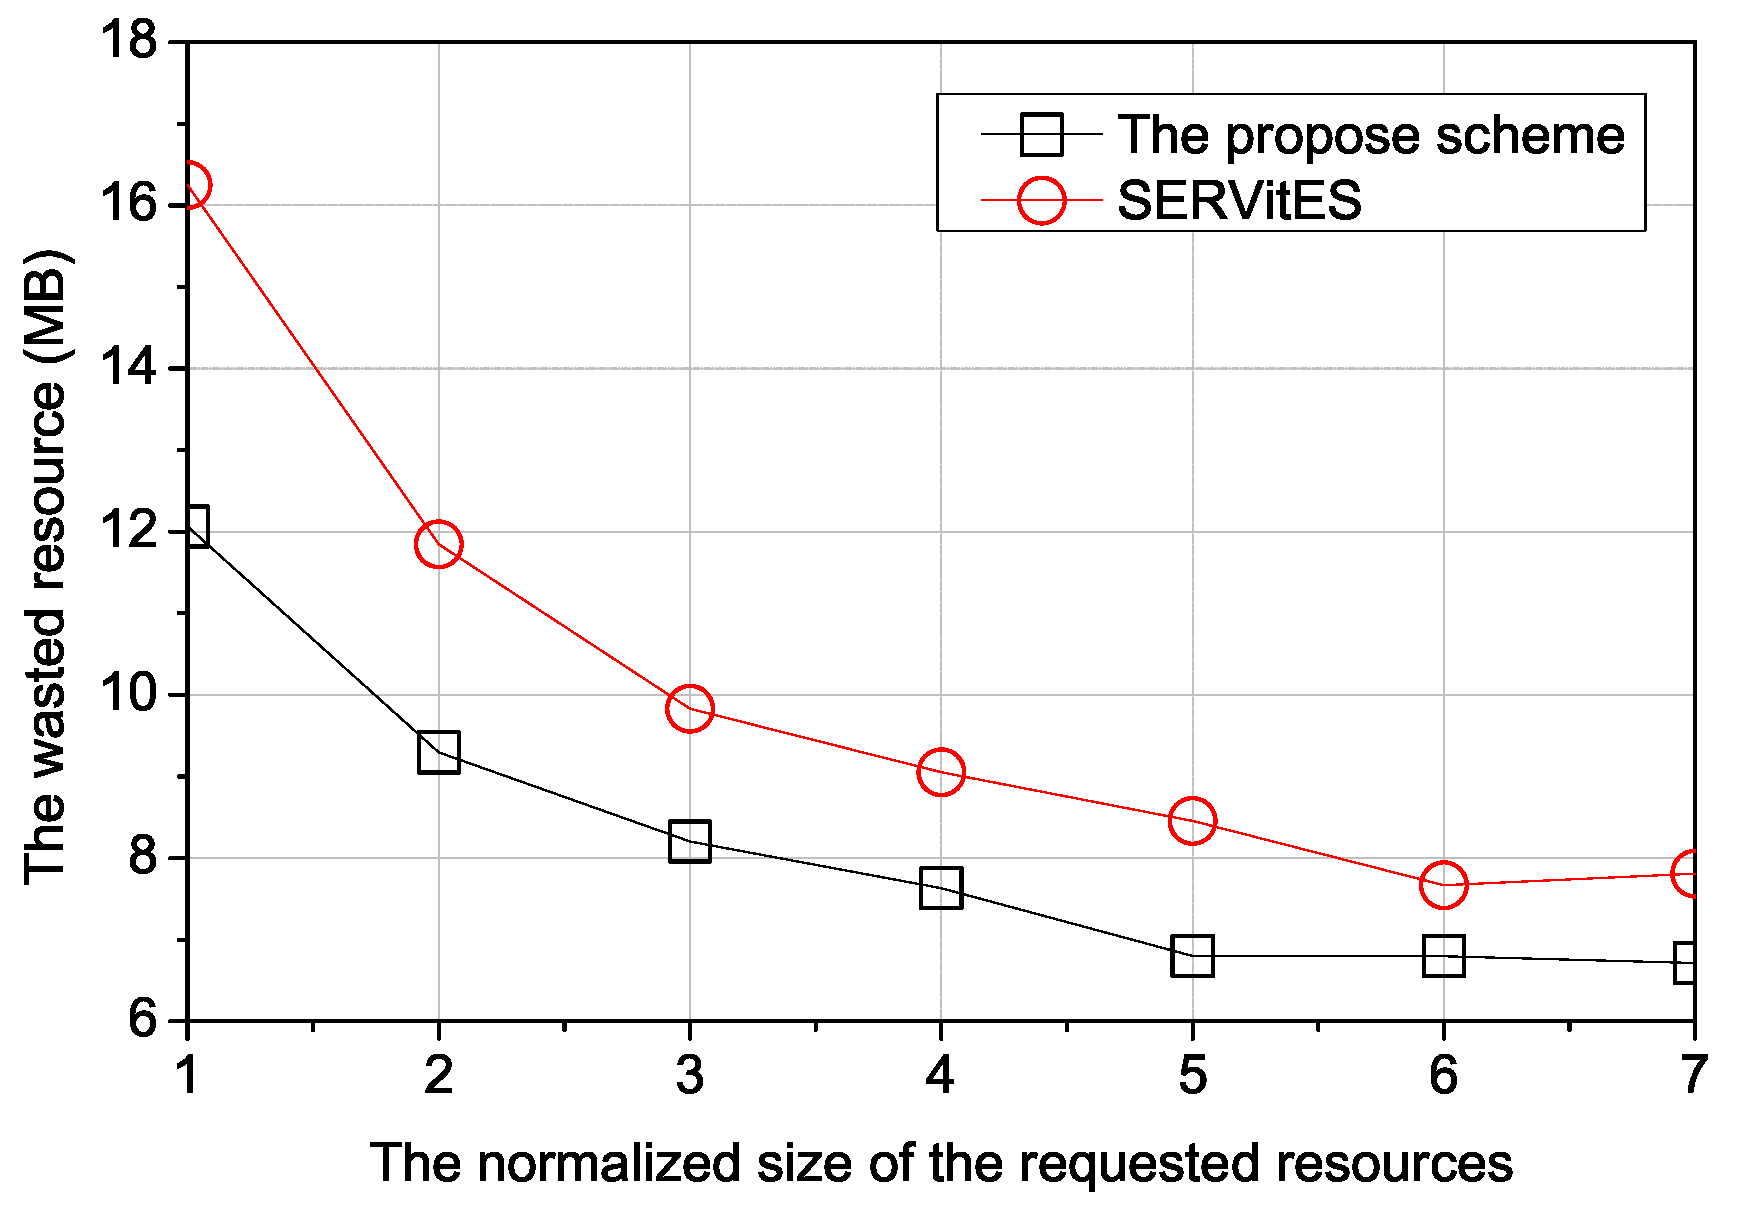
\includegraphics[width=10.5cm]{./graphs/RR.eps}
    \caption{The wasted resources for normalized sizes of requested resources.}
    \label{graph1}
\end{figure}


\begin{figure}[H]
    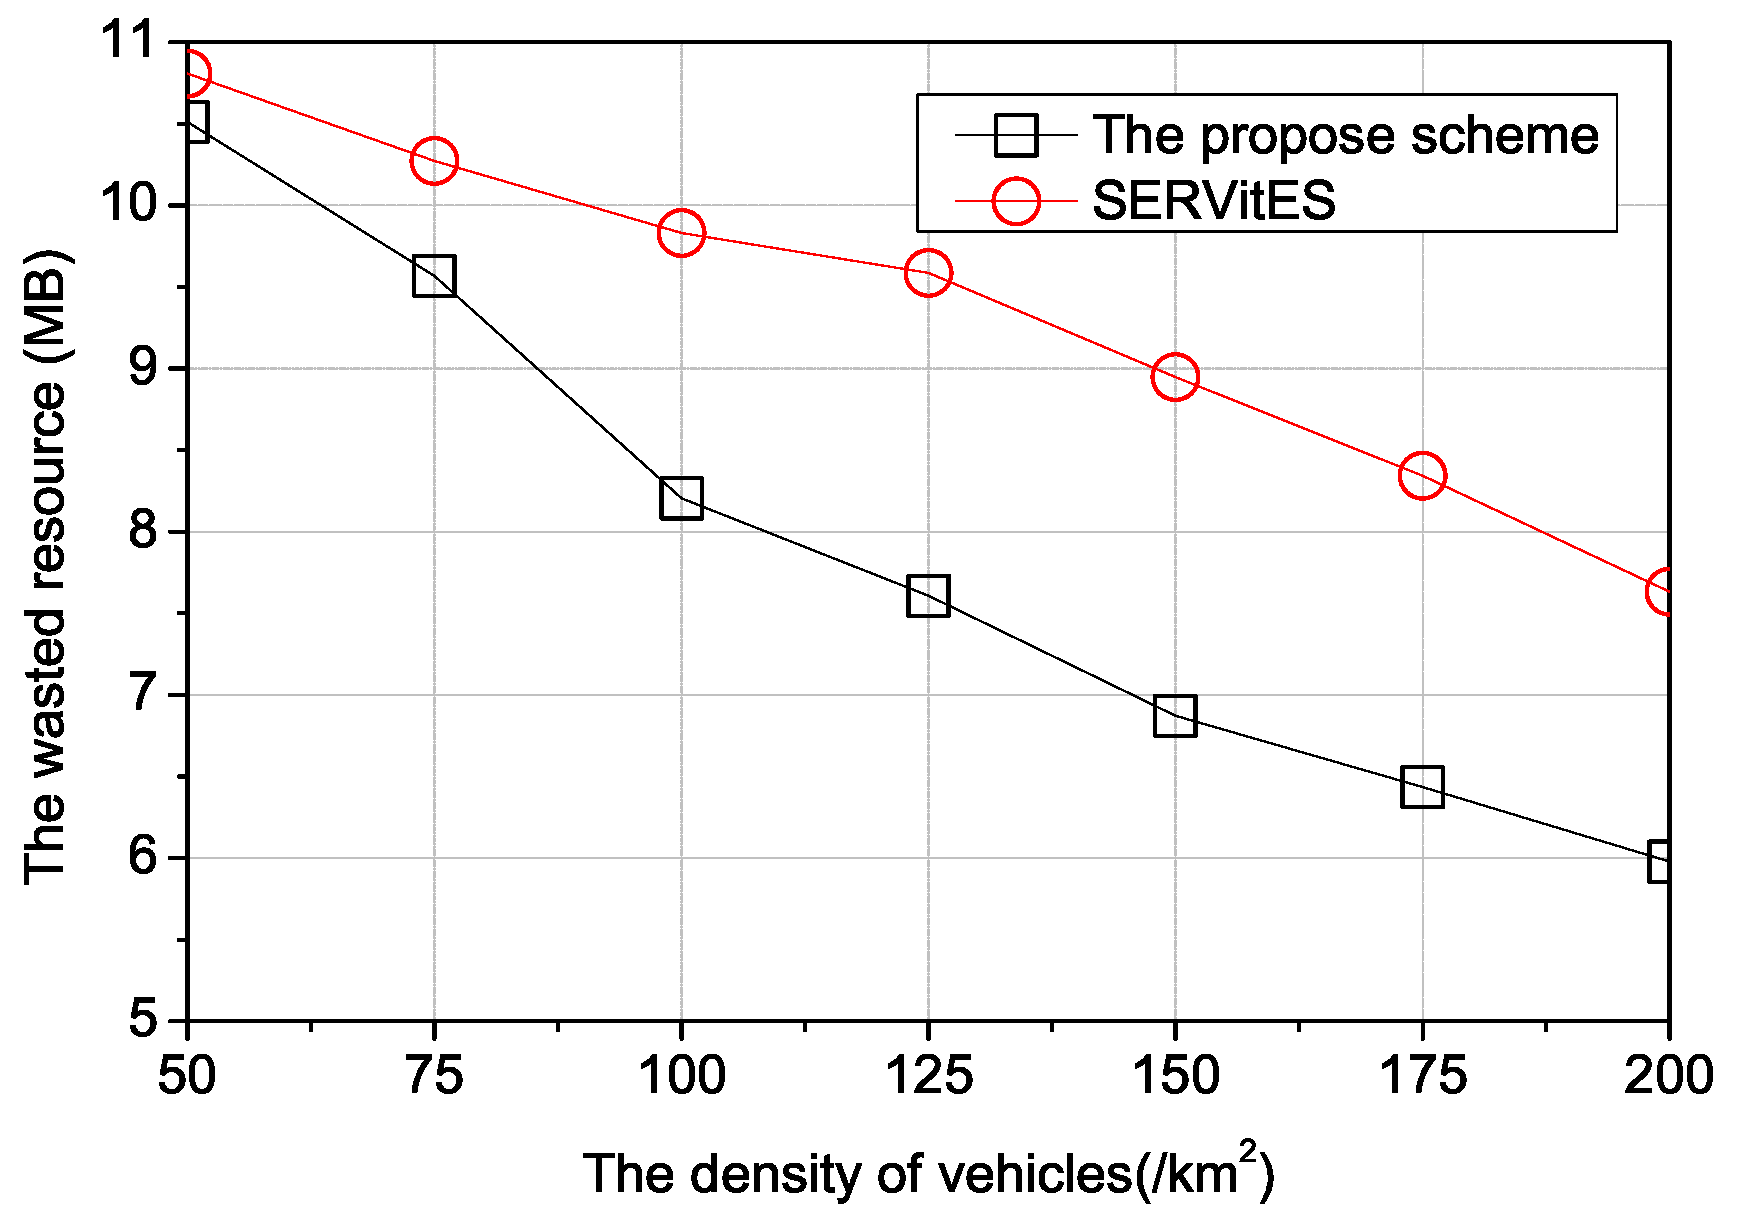
\includegraphics[width=10.5cm]{./graphs/DR.eps}
    \caption{The wasted resources according to the density of vehicles.}
    \label{graph2}
\end{figure}


Figure \ref{graph3} shows the wasted resources according to the average speed of vehicles.
Since fast vehicles suffer more intersections and may leave the vehicular cloud, their vehicular clouds need to be reconstructed more due to the low connectivity between vehicles.
To reconstruct the vehicular cloud, it is necessary to find another member vehicle instead of the leaving member vehicle that was optimally chosen.
This causes an increase in wasted resources because it may cause all the best members to get out and the worst members to be picked.
In SERVitES, more reconstruction of the vehicular cloud has a high probability that the vehicular cloud chooses a vehicle with more available resources as a member vehicle.
When frequently changing the member vehicles of the vehicular cloud, the vehicular cloud selects the vehicle with more available resources as a member vehicle, and thus, the wasted resources will be increased.
In the proposed scheme, the RSU selects the vehicle that best minimizes the wasted resources as a member vehicle.
When vehicles are slow, the optimally selected member vehicle of the vehicular cloud maintains its cloud longer.
Thus, the proposed scheme has fewer wasted resources than SERVitES.

\begin{figure}[H]
    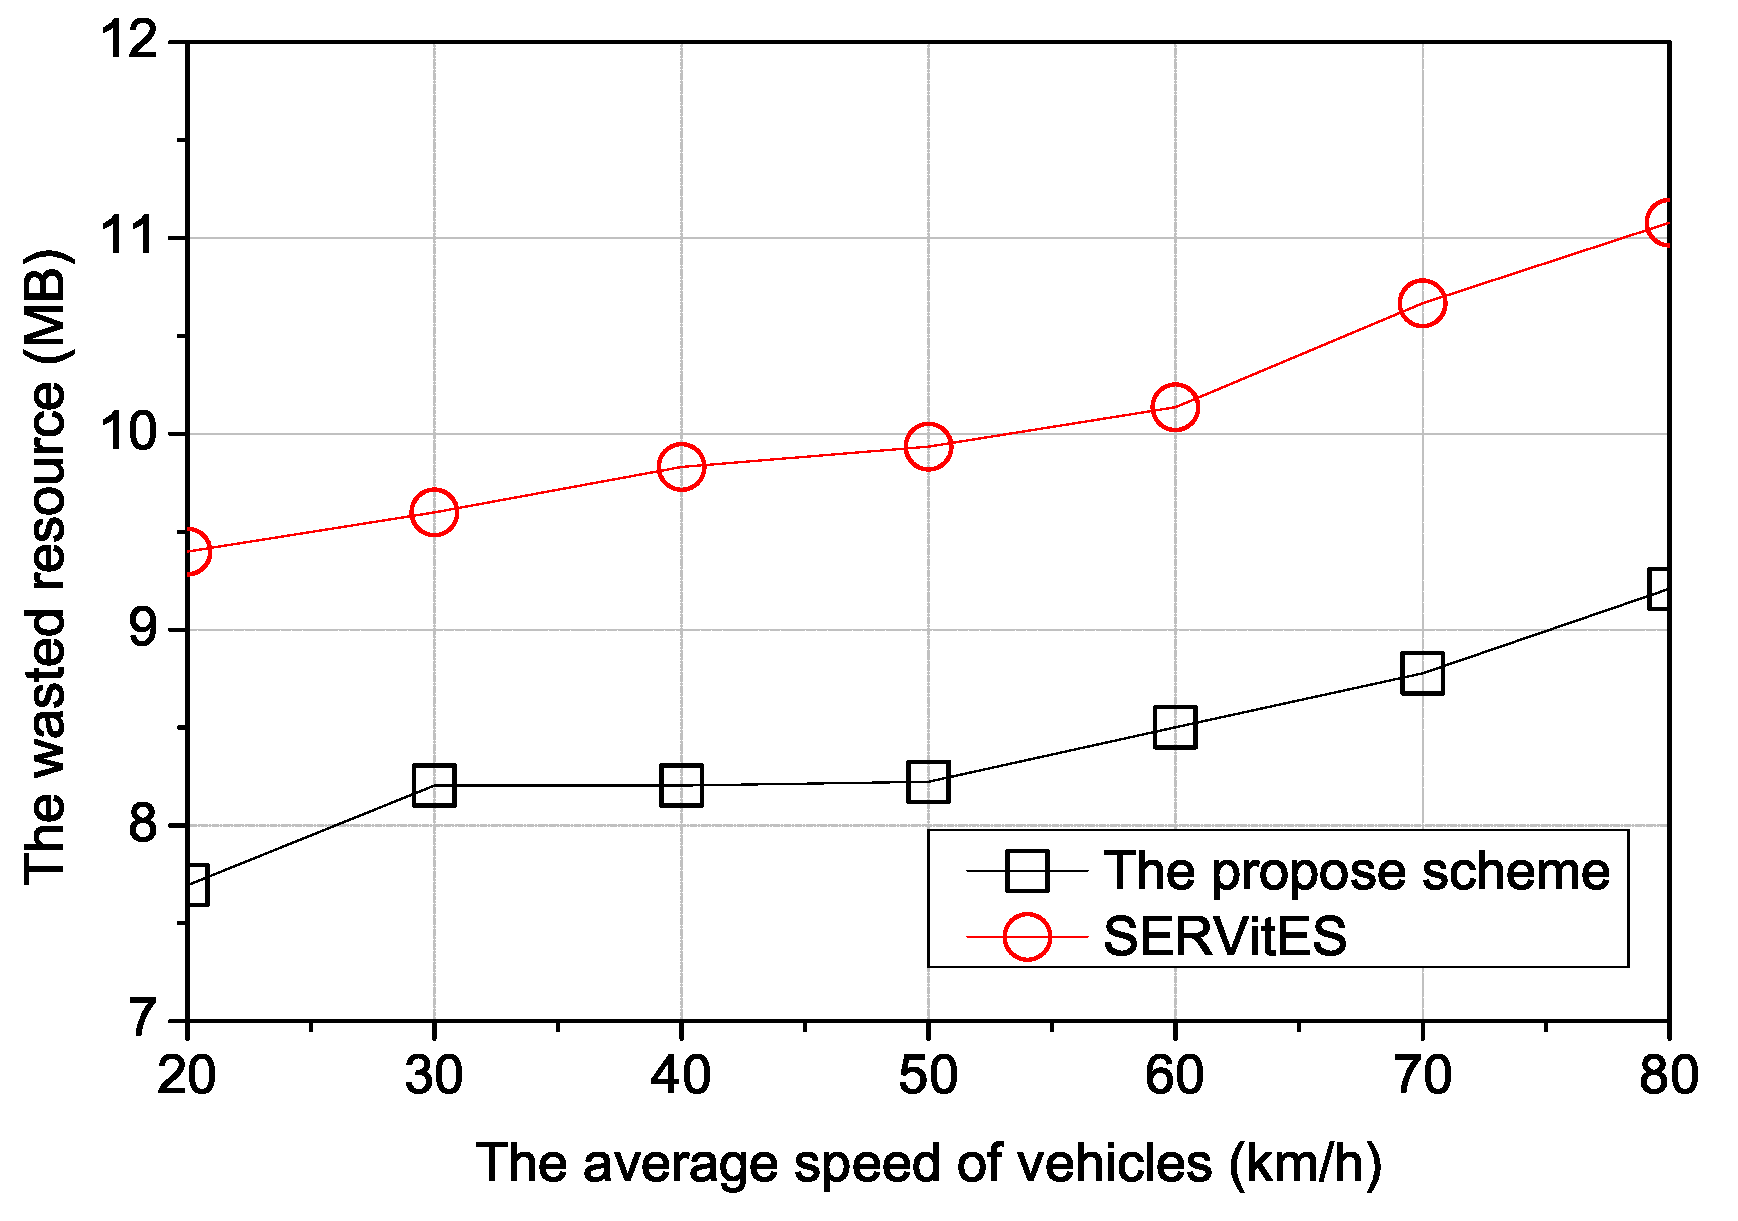
\includegraphics[width=10.5cm]{./graphs/SR.eps}
    \caption{The wasted resources according to the average speed of vehicles.}
    \label{graph3}
\end{figure}

\subsubsection{The Number of Cloud Reconstructions} \label{sec5.2.2}


Figure \ref{graph4} shows the number of cloud reconstructions according to the normalized size of the requested resources.
When the size of the requested resource is large, the vehicular cloud needs more member vehicles to maintain itself.
If the vehicular cloud includes many member vehicles, the probability that one member vehicle leaves the vehicular cloud is increased.
In that case, since the vehicular cloud is destroyed by leaving member vehicles, the vehicular cloud needs to be reconstructed.
Thus, if the size of the requested resource is large, the reconstruction of the vehicular cloud frequently occurs due to the high probability of leaving member vehicles.
In SERVitES, the vehicle with the largest amount of available resources is selected as the member vehicle of the vehicular cloud based on the current speed of the vehicle.
The connectivity between vehicles is very unstable because the vehicles can change their speed and direction in the network area.
This leads to an increased number of reconstructions necessary for the vehicular cloud.
In the proposed scheme, the prediction of the connection between the member vehicles is more accurate than SERVitES because the RSU considers the connectivity between vehicles.
Therefore, the proposed scheme has a more stable connection compared with SERVitES.


\begin{figure}[H]
    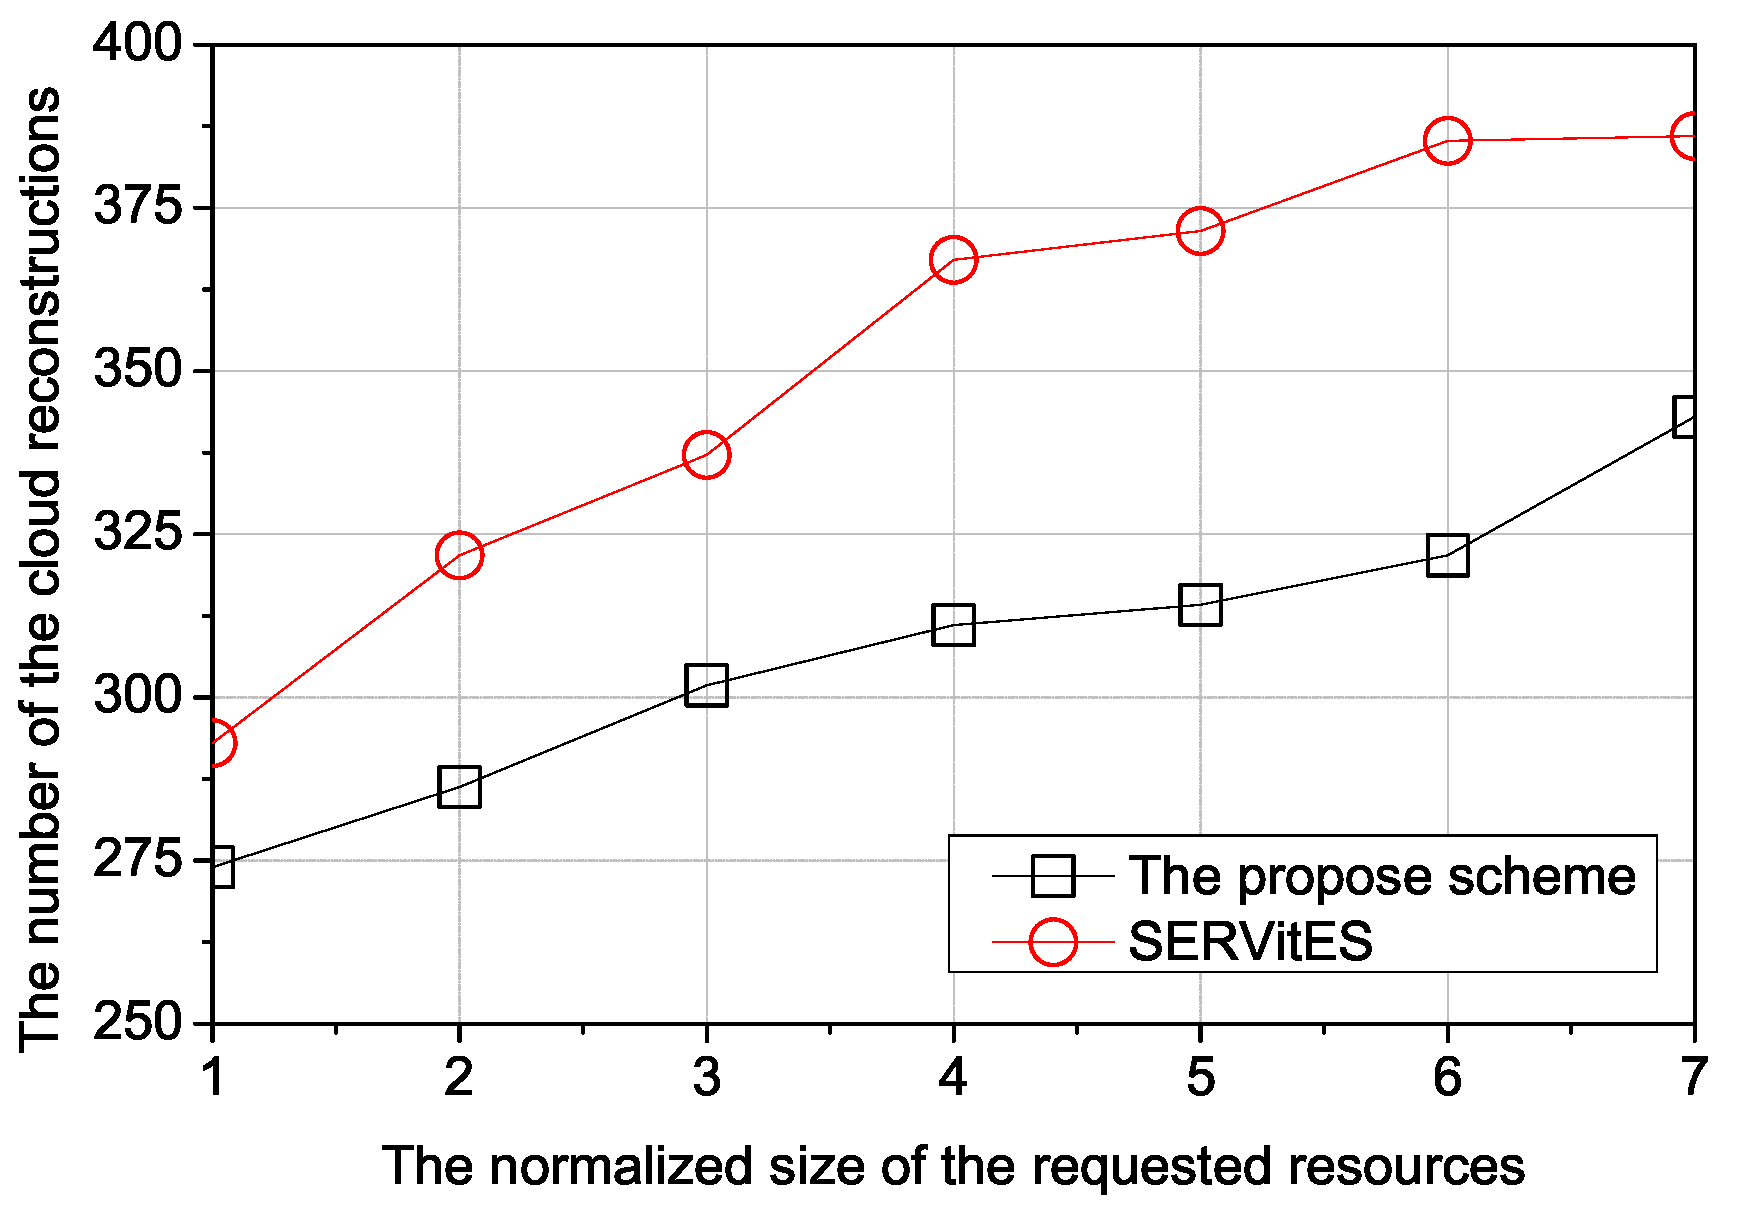
\includegraphics[width=10.5cm]{./graphs/RN.eps}
    \caption{The number of cloud reconstructions according to the normalized size of the requested resources.}
    \label{graph4}
\end{figure}


Figure \ref{graph5} shows the number of the cloud reconstructions according to the density of vehicles.
If the density of vehicles is high, the vehicular cloud can choose the best member vehicles to construct the vehicular cloud in terms of connectivity because there are more candidate vehicles that can be member vehicles.
Thus, when vehicles are dense, the member vehicles hardly leave the vehicular cloud because of enough candidate vehicles.
In SERVitES, the requester vehicle considers the connectivity between itself and the candidate vehicles to receive the largest amount of resources.
The number of the cloud reconstructions is reduced because the requester can select the vehicles that have good connectivity to the requester vehicle and large available resources when vehicles are dense.
In the proposed scheme, using a more accurate prediction of vehicle mobility, the RSU can allocate the replacement vehicle with the optimized connectivity to the requester vehicle to reconstruct the vehicular cloud.
Accordingly, the proposed scheme has fewer requests for the reconstruction of vehicular clouds than SERVitES.

\begin{figure}[H]
    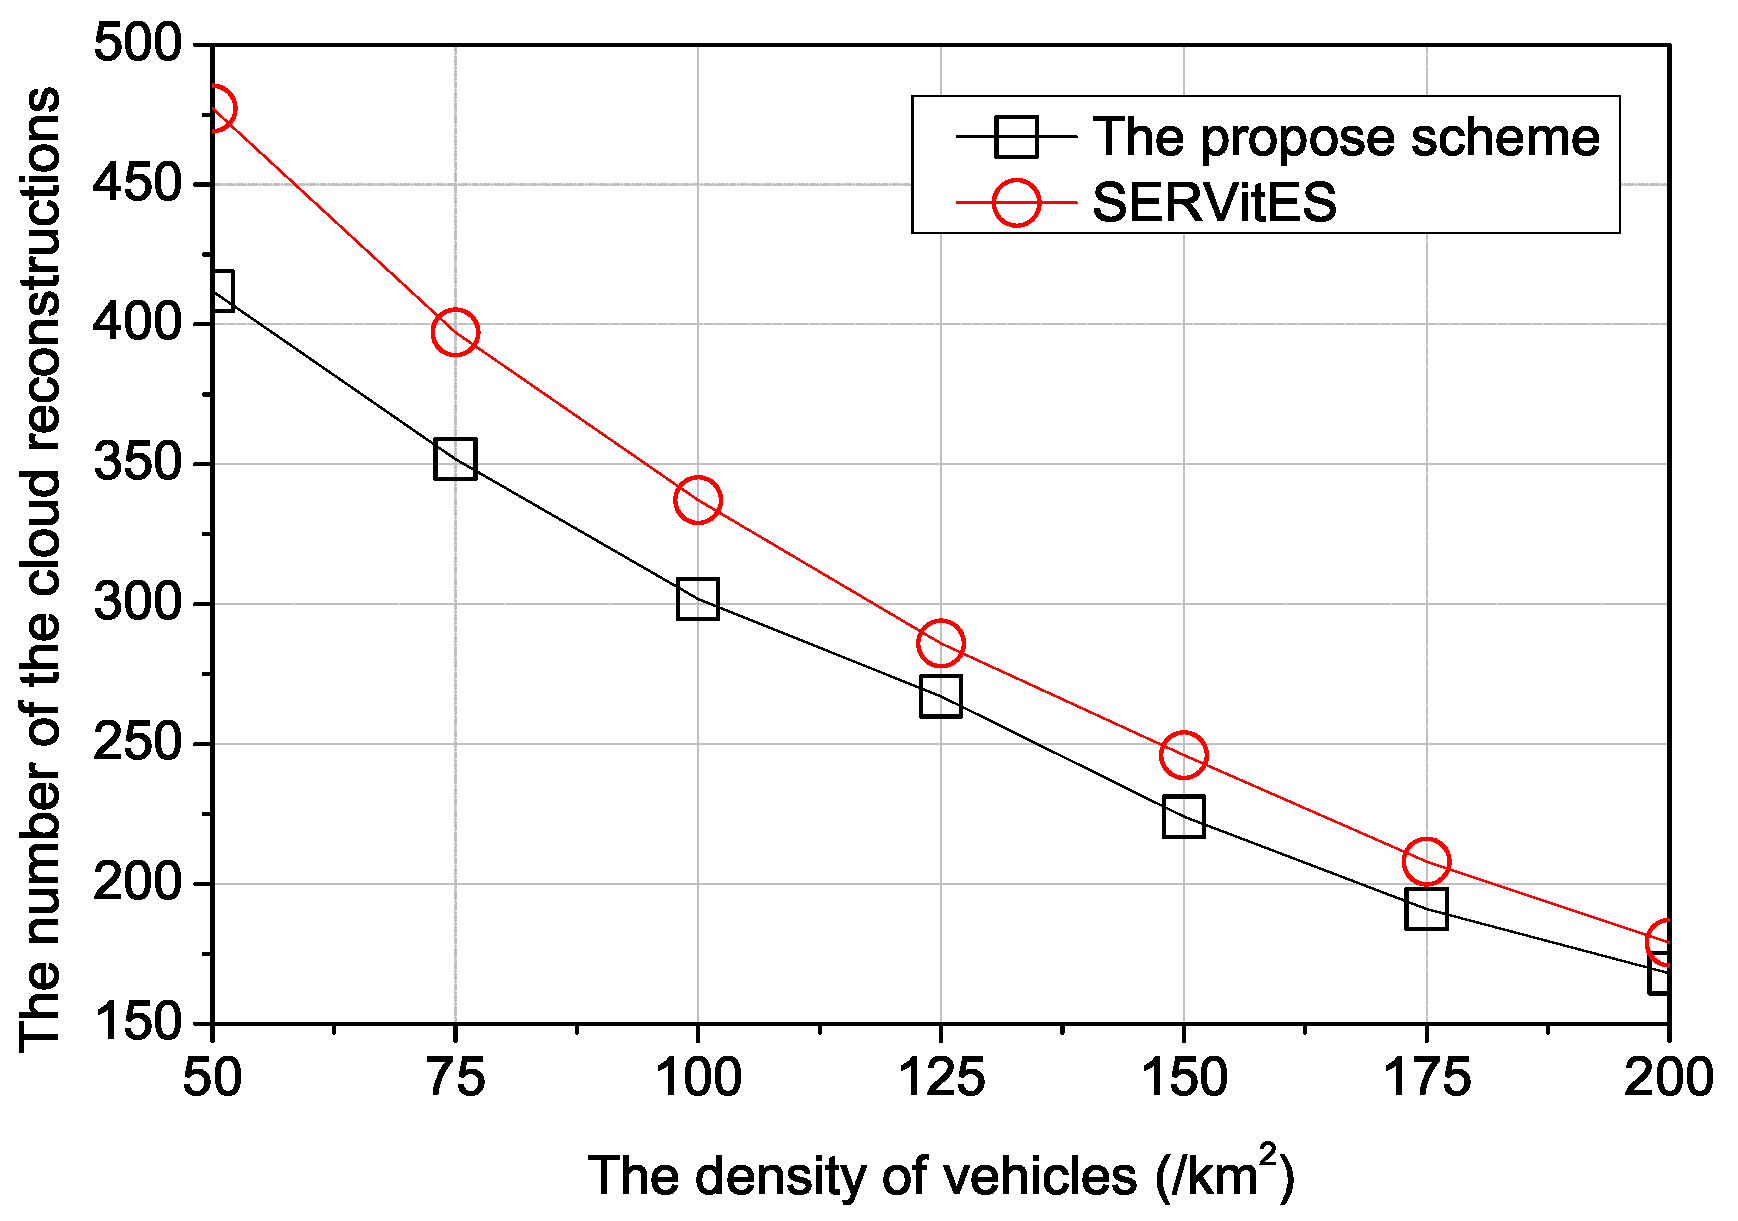
\includegraphics[width=10.5cm]{./graphs/SN.eps}
    \caption{The number of the cloud reconstructions according to the density of vehicles.}
    \label{graph5}
\end{figure}

Figure \ref{graph6} shows the number of the cloud reconstructions according to the average speed of vehicles.
When vehicles are fast, the connection time between vehicles is reduced due to suffering more intersections and leaving the vehicular cloud quickly.
The vehicular cloud needs time to maintain the connection among member vehicles to provide the available resources to the requester vehicle.
During the needed time, the vehicular cloud needs more reconstruction to maintain it due to the increased disconnection between vehicles.
In SERVitES, the requester vehicle tries to maintain the vehicular cloud by searching for a replacement vehicle in the V2V communication range.
Due to the relatively short range of communication, the number of candidate vehicles is not adequate to select the best member vehicles in terms of the connectivity.
In the proposed scheme, the vehicular cloud can replace its leaving member vehicles with the replacement vehicles using the V2I communication range.
Due to the relatively long range of communication, the number of candidate vehicles is adequate to select the optimized member vehicles in terms of connectivity and saving wasted resources.
For this reason, the proposed scheme has fewer instances of cloud reconstruction according to the average speed of vehicles.

\begin{figure}[H]
    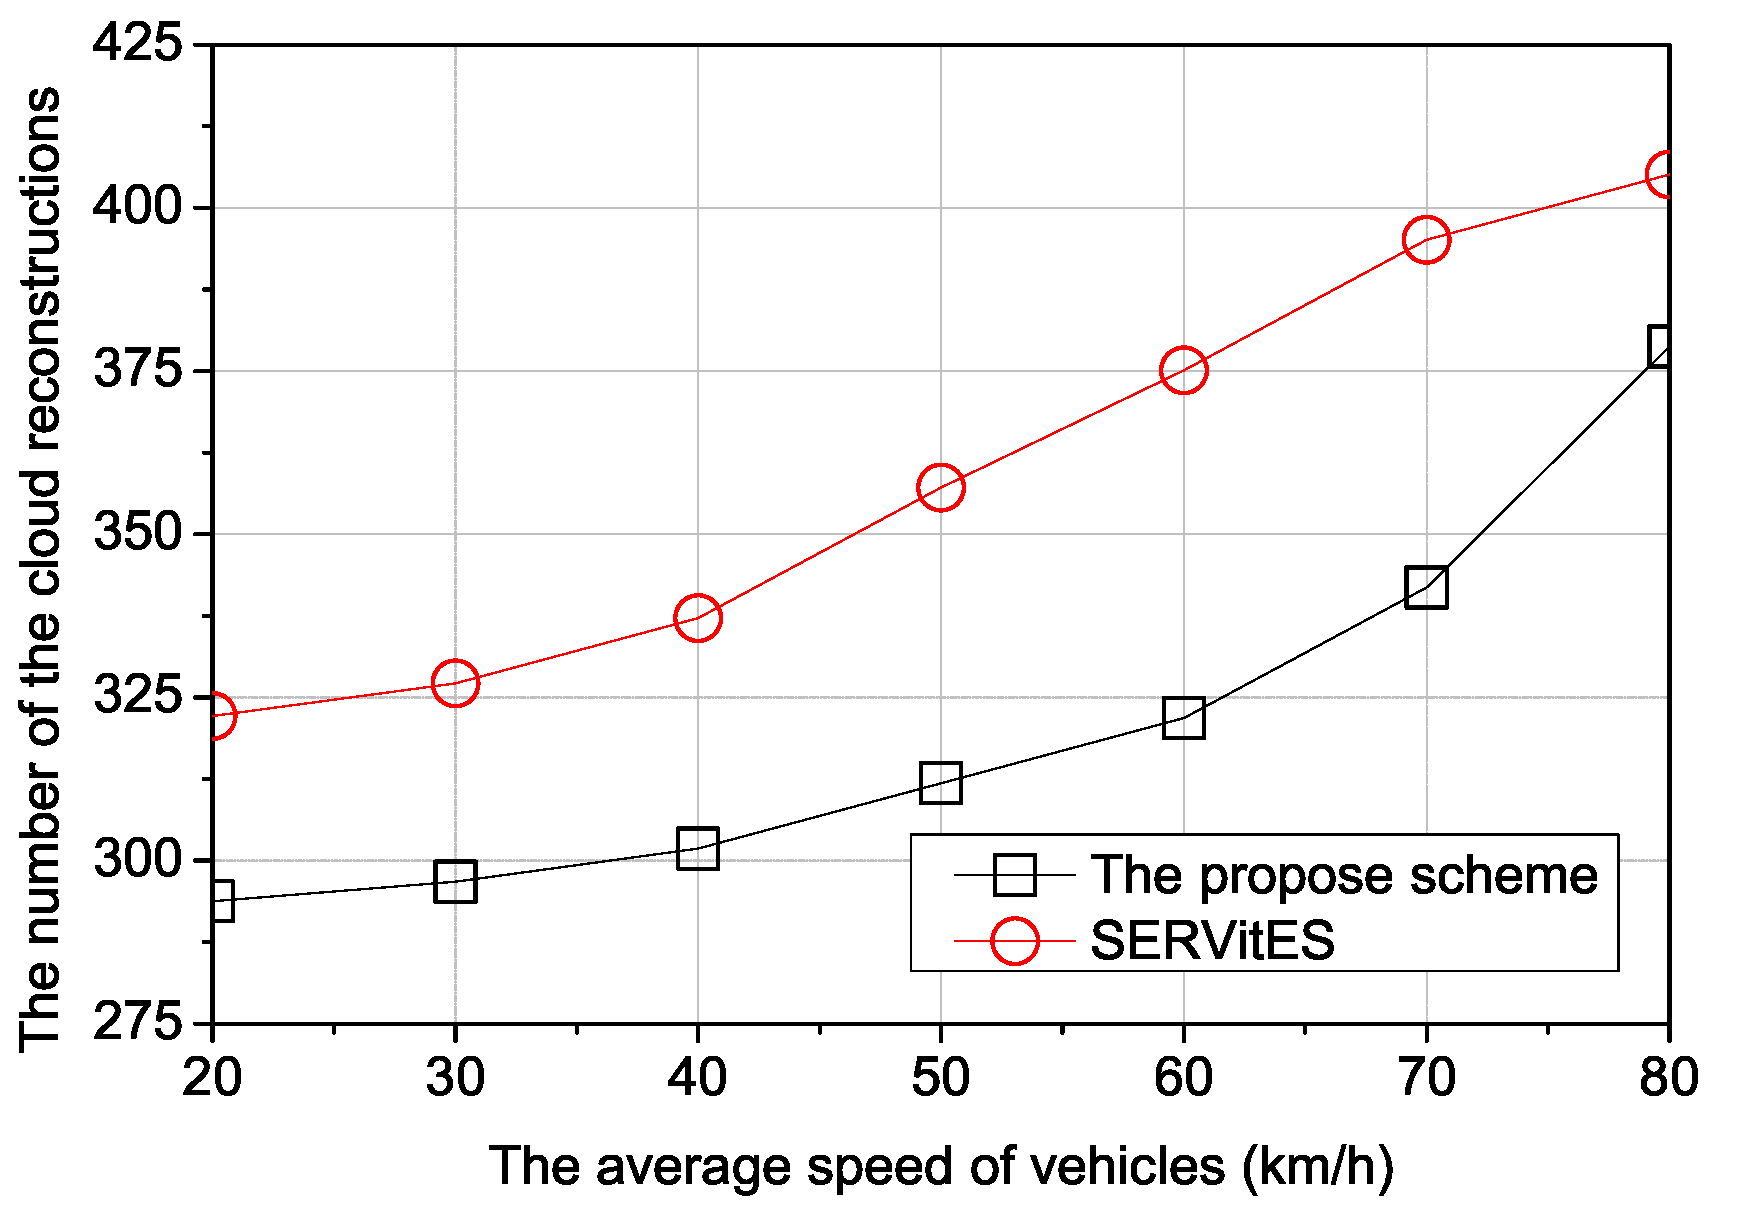
\includegraphics[width=10.5cm]{./graphs/DN.eps}
    \caption{The number of cloud reconstructions according to the average speed of vehicles.}
    \label{graph6}
\end{figure}

\section{Conclusions and Future Work} \label{con}
\subsection{Conclusions}
In this paper, we address the issue of replacing the leaving member vehicles of vehicular clouds with new member vehicles to reconstruct vehicular clouds at intersections in VANETs.
To do this, we propose an RSU-aided optimal member replacement scheme for the reconstruction of vehicular clouds in VANETs in order to reduce the number of cloud reconstructions and wasted resources.
The proposed scheme does not include RSUs as members of vehicular clouds, but only exploits their computational and coverage ability in order to determine optimal new members to replace the leaving member vehicles on intersections.
With the ability of RSUs, the proposed scheme first provides an improved mobility prediction model to enhance the connectivity prediction accuracy of vehicles in vehicular clouds.
Our improved mobility prediction model considers both the mobility 
prediction based on Gaussian probability and the trajectory prediction based on a Markov model and calculates the probability of the connection of vehicles in one and multiple directions.
Next, the proposed scheme presents the problem of identifying optimal replacement member vehicles to minimize the wasted resources of vehicles,
which is formulated by the ratio of the size of the requested resource and the available resources of the vehicles.
Then, the problem is solved through integer linear programming (ILP) in order to achieve minimization of the wasted resources.
To evaluate the performance of the proposed scheme, we implement a simulation using NS3 with the enhanced Manhattan mobility model, wherein vehicles accelerate with a Gaussian distribution and conduct directional shifts with the Markov model on the road.
Simulation results verified that the proposed scheme achieves smaller numbers of cloud reconstruction and fewer wasted resources compared with SERVitES.

\subsection{Future Work}
The proposed scheme selects the optimal replacement member vehicles to minimize wasted resources with the stable connectivity of a vehicular cloud in a restricted environment for the fairness of wireless resources and energies.
However, it has a limitation regarding the prediction failure due to unexpected situations such as accidents, changes in the driver's mind, etc.
After detecting the failure of the mobility prediction, we can solve that problem by using other optimization models or machine learning.
Additionally, the mobility prediction of vehicles can be improved by using machine learning in real scenarios.
Therefore, we will handle the prediction failure due to unexpected situations and improve the accuracy of the vehicle mobility prediction to enhance the performance of the proposed scheme in real scenarios.


% In VANET, we propose a scheme to minimize the wasted resource in the reconstruction process for maintaining the vehicular cloud by utilizing information from small computational resources and neighbors in the RSU. While the vehicular cloud is suggested to alleviate the overhead of RSUs, it undergoes frequent reconstruction due to the irregular mobility of vehicles. Furthermore, because early generated vehicular clouds preempt good resources due to not considering the wasted resource, new requester vehicles do not reliably construct the vehicular clouds. Accordingly, we first secure sufficient candidate vehicles by using the neighbor vehicles' information of the RSU. In addition, utilizing RSU's small computing resources, the combination of the location prediction for vehicles using the Gaussian distribution and the trajectory prediction for vehicles using the Markov Model reduces the reconstruction of the vehicular cloud by selecting vehicles that have the high connectivity as a replacement vehicle. Also, by minimizing the wasted resource, stability for the construction of the entire requester vehicle is improved. We demonstrate that the proposed scheme minimizes the wasted resource compared to the SERVitES by implementing an improved Manhattan Mobility Model with the directional shift of the vehicle along with the Markov Model and the mobility of the vehicle along with the Gaussian distribution.

%\section{Patents}
%This section is not mandatory, but may be added if there are patents resulting from the work reported in this manuscript.
%%%%%%%%%%%%%%%%%%%%%%%%%%%%%%%%%%%%%%%%%%
\vspace{6pt}
%%%%%%%%%%%%%%%%%%%%%%%%%%%%%%%%%%%%%%%%%%
%% optional
%\supplementary{The following supporting information can be downloaded at:  \linksupplementary{s1}, Figure S1: title; Table S1: title; Video S1: title.}

% Only for the journal Methods and Protocols:
% If you wish to submit a video article, please do so with any other supplementary material.
% \supplementary{The following supporting information can be downloaded at: \linksupplementary{s1}, Figure S1: title; Table S1: title; Video S1: title. A supporting video article is available at doi: link.}
%%%%%%%%%%%%%%%%%%%%%%%%%%%%%%%%%%%%%%%%%%
\authorcontributions{Conceptualization, H.C.; methodology, Y.N.; software, Y.N.; validation, H.C., Y.S. and D.M.; writing---original draft preparation, Y.N.; writing---review and editing, H.C. and E.L.; supervision, E.L.; funding acquisition, E.L. All authors have read and agreed to the published version of the~manuscript.}

\funding{\hl{This research was supported by Basic Science Research Program through the National Research Foundation of Korea (NRF) funded by the Ministry of Education (NRF-2018R1D1A3B07042838).} %MDPI: please confirm the suggest change.
}
\institutionalreview{Not applicable.}
\informedconsent{Not applicable.}
\dataavailability{Not applica\hl{ble.} %MDPI: we delete Acknowledgement part, please confirm.
}
\conflictsofinterest{The authors declare no conflict of~interest.}
%%%%%%%%%%%%%%%%%%%%%%%%%%%%%%%%%%%%%%%%%%
%% Only for journal Encyclopedia
%\entrylink{The Link to this entry published on the encyclopedia platform.}
%%%%%%%%%%%%%%%%%%%%%%%%%%%%%%%%%%%%%%%%%%
%% Optional
\appendixtitles{no} % Leave argument "no" if all appendix headings stay EMPTY (then no dot is printed after "Appendix A"). If the appendix sections contain a heading then change the argument to "yes".

%\section[\appendixname~\thesection]{}
%All appendix sections must be cited in the main text. In the appendices, Figures, Tables, etc. should be labeled, starting with ``A''---e.g., Figure A1, Figure A2, etc.
%%%%%%%%%%%%%%%%%%%%%%%%%%%%%%%%%%%%%%%%%%
\begin{adjustwidth}{-\extralength}{0cm}
\reftitle{References} \begin{thebibliography}{999}
\bibitem{zhang2020}
Zhang, Z.; Lung, C.-H.; St-Hilaire, M.; Lambadaris, I.  Smart Proactive Caching: Empower the Video Delivery for Autonomous Vehicles in ICN-Based Networks. \textit{IEEE Trans. Veh. Technol.} \textbf{2020}, \emph{69},  7955--7965. https://doi.org/10.1109/TVT.2020.2994181.

\bibitem{yuan2018}
Yuan, Q.; Zhou, H.; Li, J.; Liu, Z.; Yang, F.; Shen, X.S.  Toward Efficient Content Delivery for Automated Driving Services: An Edge Computing Solution. \textit{IEEE Netw.} \textbf{2018}, \emph{32}, 80--86. https://doi.org/10.1109/MNET.2018.1700105.


\bibitem{Meneguette2017j}
Meneguette, R.I.; Boukerche, A. SERVitES: An efficient search and allocation resource protocol based on V2V communication for vehicular cloud. \textit{Comput. Netw.} \textbf{2017},  \emph{123}, 104-118. https://doi.org/10.1016/j.comnet.2017.05.014.


% V2I
\bibitem{Lee2019}
Lee, Y.; Choi, H.; Nam, Y.; Park, S.; Lee, E. RSU-driven Cloud Construction and Management Mechanism in VANETs. In Proceedings of the {2019 IEEE 8th International Conference on Cloud Networking (CloudNet)}, \hl{Coimbra, Portugal, 4--6 November} 2019; pp. 1--4. https://doi.org/10.1109/CloudNet47604.2019.9064111.

\bibitem{Lin2017}
Lin, C.-C.; Deng, D.-J.; Yao, C.-C. Resource Allocation in Vehicular Cloud Computing Systems With Heterogeneous Vehicles and Roadside Units. \textit{IEEE Internet Things J.} \textbf{2018}, \emph{5}, 3692--3700. https://doi.org/10.1109/JIOT.2017.2690961.

% V2V
\bibitem{Sibai2015}
Sibaï, R.E.; Atéchian, T.; Abdo, J.B.; Tawil, R.; Demerjian, J.  Connectivity-aware service provision in vehicular cloud. In Proceedings of the {2015 International Conference on Cloud Technologies and Applications (CloudTech)}, \hl{Marrakesh, Morocco, 2--4 June } %MDPI: We added the location and date of the conference. Please confirm.
  2015; pp. 1--5. https://doi.org/10.1109/CloudTech.2015.7337017.

\bibitem{Meneguette2016}
Meneguette, R.I.; Boukerche, A.; de Grande, R.  SMART: An Efficient Resource Search and Management Scheme for Vehicular Cloud-Connected System. In Proceedings of the {2016 IEEE Global Communications Conference (GLOBECOM)}, \hl{Washington, DC, USA, 4--8 December} 2016; pp. 1--6. https://doi.org/10.1109/GLOCOM.2016.7842271.

\bibitem{Meneguette2017b}
Meneguette, R.I.; Boukerche, A.  Peer-to-Peer Protocol for Allocated Resources in Vehicular Cloud Based on V2V Communication. In Proceedings of the {2017 IEEE Wireless Communications and Networking Conference (WCNC)}, \hl{San Francisco, CA, USA, 19--22 March} 2017; pp. 1--6. https://doi.org/10.1109/WCNC.2017.7925602.

\bibitem{Meneguette2017}
Meneguette, R.I.; Boukerche, A. A cooperative and adaptive resource scheduling for Vehicular Cloud. In Proceedings of the {2017 IEEE Symposium on Computers and Communications (ISCC)}, \hl{Heraklion, Greece, 3--6 July} 2017; pp. 398-403. https://doi.org/10.1109/ISCC.2017.8024562.


\bibitem{Choi2018}
Choi, H.; Nam, Y.; Bang, J.; Lee, E.  Multi-hop Vehicular Cloud Construction with Connection Time based Resource Allocation in VANETs. In Proceedings of the {2018 24th Asia-Pacific Conference on Communications (APCC)}, \hl{Ningbo, China, 12--14 November} 2018; pp. 100--105. https://doi.org/10.1109/APCC.2018.8633558.


\bibitem{Mershad2013}
Mershad, K.; Artail, H.  Finding a star in a vehicular cloud. \textit{IEEE Intell. Transp. Syst. Mag.} \textbf{2013},  5, 55--68. https://doi.org/ 10.1109/MITS.2013.2240041.

\bibitem{Mershad2013j}
Mershad, K.; Artail, H.  Crown: Discovering and consuming services in vehicular clouds. In Proceedings of the {2013 Third International Conference on Communications and Information Technology (ICCIT)}, \hl{Beirut, Lebanon, 19--21 June} 2013; pp. 98--102. https://doi.org/10.1109/ICCITechnology.2013.6579530.

\bibitem{Yu2013}
Yu, R.; Zhang, Y.; Gjessing, S.; Xia, W.; Yang, K.  Toward cloud-based vehicular networks with efficient resource management. \textit{IEEE Netw.} \textbf{2013}, \emph{27}, 48--55. https://doi.org/10.1109/MNET.2013.6616115.



\bibitem{Salahuddin2014}
Salahuddin, M.A.; Al-Fuqaha, A.; Guizani, M.; Cherkaoui, S.  RSU cloud and its resource management in support of enhanced vehicular applications. In Proceedings of the {2014 IEEE Globecom Workshops (GC Wkshps)}, \hl{Austin, TX, USA, 8--12 December} 2014; pp. 127--132. https://doi.org/10.1109/GLOCOMW.2014.7063418.

\bibitem{Gao2018}
Gao, Z.; Chen, D.; Cai, S.; Wu, H.-C.  Optimal and Greedy Algorithms for the One-Dimensional RSU Deployment Problem With New Model.  \emph{IEEE Trans. Veh. Technol.} \textbf{2018}, \emph{67}, 7643--7657. https://doi.org/10.1109/TVT.2018.2837033.


\bibitem{Abdelhamid2017}
Abdelhamid, S.; Benkoczi, R.; Hassanein, H.S.  Vehicular clouds:Ubiquitous computing on wheels. In \textit{Emergent Computation}; Springer: Cham, Switzerland,  2017, pp. 435--452. https://doi.org/10.1007/978-3-319-46376-6\_20.

\bibitem{Jaiboon2017}
Jaiboon, V.; Thaenthong, J. Infotainment data dissemination mechanism using RSU cloud based for vehicular networks. In Proceedings of the {2017 9th International Conference on Information Technology and Electrical Engineering (ICITEE)}, \hl{Phuket, Thailand, 12--13 October} 2017; pp. 1--6. https://doi.org/10.1109/ICITEED.2017.8250450.

\bibitem{Elahi2021}
Elahi, M.M.; Rahman, M.M.; Islam, M.M.  RSU-aided Mobility-aware Dynamic Resource Allocation for Vehicular Cloud Services. In Proceedings of the {2021 International Conference on Software Engineering \& Computer Systems and 4th International Conference on Computational Science and Information Management (ICSECS-ICOCSIM)}, \hl{Pekan, Malaysia, 24--26 August} 2021; pp. 493--498. https://doi.org/10.1109/ICSECS52883.2021.00096.

\bibitem{Rahman2018}
Rahman, F.H.; Wan, A.T.; Newaz, S.H.S.; Suhaili, W.S.  Vehicular Clustering: Fog Paradigm and Recent Advances. In Proceedings of the {2018 IEEE 18th International Conference on Communication Technology (ICCT)}, \hl{Chongqing, China, 8--11 October} 2018; pp.~468--472. https://doi.org/10.1109/ICCT.2018.8600255.


\bibitem{Yu2022}
Yu, H.; Liu, R.; Li, Z.; Ren, Y.; Jiang, H. An RSU Deployment Strategy Based on Traffic Demand in Vehicular Ad Hoc Networks (VANETs).  \emph{IEEE Internet Things J.} \textbf{2022},  \emph{9}, 6496--6505. https://doi.org/10.1109/JIOT.2021.3111048.

\bibitem{Robert2018}
Krajewski, R.; Bock, J.; Kloeker, L.; Eckstein, L. The highD Dataset: A Drone Dataset of Naturalistic Vehicle Trajectories on German Highways for Validation of Highly Automated Driving Systems. In Proceedings of the {2018 IEEE 21st International Conference on Intelligent Transportation Systems (ITSC)}, \hl{Maui, HI, USA, 4--7 November} 2018. https://doi.org/10.48550/arXiv.1810.05642

\bibitem{Yen2020} % [-5,5]m/s^2
Yen, Y.-T.; Chou, J.-J.; Shih, C.-S.; Chen, C.-W.; Tsung, P.-K. Proactive Car-Following Using Deep-Reinforcement Learning. In Proceedings of the  {2020 IEEE 23rd International Conference on Intelligent Transportation Systems (ITSC)}, \hl{Rhodes, Greece, 20--23 September} 2020; pp. 1--6. https://doi.org/10.1109/ITSC45102.2020.9294194.

\bibitem{jiang2019}
Jiang, M.; Zhang, Q.; Feng, Z.; Han, Z.; Li, W. Mobility Prediction Based Virtual Routing for Ad Hoc UAV Network. In Proceedings of the {2019 IEEE Global Communications Conference (GLOBECOM)}, \hl{Waikoloa, HI, USA, 9--13 December} 2019; pp.~1--6. https://doi.org/10.1109/GLOBECOM38437.2019.9014182.

\bibitem{lin2012} 
Lin, L.; Sun, Q.; Wang, S.; Yang, F. A geographic mobility prediction routing protocol for Ad Hoc UAV Network. In Proceedings of the {2012 IEEE Globecom Workshops},  \hl{Anaheim, CA, USA, 3--7 December} 2012; pp. 1597--1602. https://doi.org/10.1109/GLOCOMW.2012.6477824.

\end{thebibliography}
\end{adjustwidth}

\end{document}